\documentclass[11pt]{article}

    \usepackage[breakable]{tcolorbox}
    \usepackage{parskip} % Stop auto-indenting (to mimic markdown behaviour)
    
    \usepackage{iftex}
    \ifPDFTeX
    	\usepackage[T1]{fontenc}
    	\usepackage{mathpazo}
    \else
    	\usepackage{fontspec}
    \fi

    % Basic figure setup, for now with no caption control since it's done
    % automatically by Pandoc (which extracts ![](path) syntax from Markdown).
    \usepackage{graphicx}
    % Maintain compatibility with old templates. Remove in nbconvert 6.0
    \let\Oldincludegraphics\includegraphics
    % Ensure that by default, figures have no caption (until we provide a
    % proper Figure object with a Caption API and a way to capture that
    % in the conversion process - todo).
    \usepackage{caption}
    \DeclareCaptionFormat{nocaption}{}
    \captionsetup{format=nocaption,aboveskip=0pt,belowskip=0pt}

    \usepackage[Export]{adjustbox} % Used to constrain images to a maximum size
    \adjustboxset{max size={0.9\linewidth}{0.9\paperheight}}
    \usepackage{float}
    \floatplacement{figure}{H} % forces figures to be placed at the correct location
    \usepackage{xcolor} % Allow colors to be defined
    \usepackage{enumerate} % Needed for markdown enumerations to work
    \usepackage{geometry} % Used to adjust the document margins
    \usepackage{amsmath} % Equations
    \usepackage{amssymb} % Equations
    \usepackage{textcomp} % defines textquotesingle
    % Hack from http://tex.stackexchange.com/a/47451/13684:
    \AtBeginDocument{%
        \def\PYZsq{\textquotesingle}% Upright quotes in Pygmentized code
    }
    \usepackage{upquote} % Upright quotes for verbatim code
    \usepackage{eurosym} % defines \euro
    \usepackage[mathletters]{ucs} % Extended unicode (utf-8) support
    \usepackage{fancyvrb} % verbatim replacement that allows latex
    \usepackage{grffile} % extends the file name processing of package graphics 
                         % to support a larger range
    \makeatletter % fix for grffile with XeLaTeX
    \def\Gread@@xetex#1{%
      \IfFileExists{"\Gin@base".bb}%
      {\Gread@eps{\Gin@base.bb}}%
      {\Gread@@xetex@aux#1}%
    }
    \makeatother

    % The hyperref package gives us a pdf with properly built
    % internal navigation ('pdf bookmarks' for the table of contents,
    % internal cross-reference links, web links for URLs, etc.)
    \usepackage{hyperref}
    % The default LaTeX title has an obnoxious amount of whitespace. By default,
    % titling removes some of it. It also provides customization options.
    \usepackage{titling}
    \usepackage{longtable} % longtable support required by pandoc >1.10
    \usepackage{booktabs}  % table support for pandoc > 1.12.2
    \usepackage[inline]{enumitem} % IRkernel/repr support (it uses the enumerate* environment)
    \usepackage[normalem]{ulem} % ulem is needed to support strikethroughs (\sout)
                                % normalem makes italics be italics, not underlines
    \usepackage{mathrsfs}
    

    
    % Colors for the hyperref package
    \definecolor{urlcolor}{rgb}{0,.145,.698}
    \definecolor{linkcolor}{rgb}{.71,0.21,0.01}
    \definecolor{citecolor}{rgb}{.12,.54,.11}

    % ANSI colors
    \definecolor{ansi-black}{HTML}{3E424D}
    \definecolor{ansi-black-intense}{HTML}{282C36}
    \definecolor{ansi-red}{HTML}{E75C58}
    \definecolor{ansi-red-intense}{HTML}{B22B31}
    \definecolor{ansi-green}{HTML}{00A250}
    \definecolor{ansi-green-intense}{HTML}{007427}
    \definecolor{ansi-yellow}{HTML}{DDB62B}
    \definecolor{ansi-yellow-intense}{HTML}{B27D12}
    \definecolor{ansi-blue}{HTML}{208FFB}
    \definecolor{ansi-blue-intense}{HTML}{0065CA}
    \definecolor{ansi-magenta}{HTML}{D160C4}
    \definecolor{ansi-magenta-intense}{HTML}{A03196}
    \definecolor{ansi-cyan}{HTML}{60C6C8}
    \definecolor{ansi-cyan-intense}{HTML}{258F8F}
    \definecolor{ansi-white}{HTML}{C5C1B4}
    \definecolor{ansi-white-intense}{HTML}{A1A6B2}
    \definecolor{ansi-default-inverse-fg}{HTML}{FFFFFF}
    \definecolor{ansi-default-inverse-bg}{HTML}{000000}

    % commands and environments needed by pandoc snippets
    % extracted from the output of `pandoc -s`
    \providecommand{\tightlist}{%
      \setlength{\itemsep}{0pt}\setlength{\parskip}{0pt}}
    \DefineVerbatimEnvironment{Highlighting}{Verbatim}{commandchars=\\\{\}}
    % Add ',fontsize=\small' for more characters per line
    \newenvironment{Shaded}{}{}
    \newcommand{\KeywordTok}[1]{\textcolor[rgb]{0.00,0.44,0.13}{\textbf{{#1}}}}
    \newcommand{\DataTypeTok}[1]{\textcolor[rgb]{0.56,0.13,0.00}{{#1}}}
    \newcommand{\DecValTok}[1]{\textcolor[rgb]{0.25,0.63,0.44}{{#1}}}
    \newcommand{\BaseNTok}[1]{\textcolor[rgb]{0.25,0.63,0.44}{{#1}}}
    \newcommand{\FloatTok}[1]{\textcolor[rgb]{0.25,0.63,0.44}{{#1}}}
    \newcommand{\CharTok}[1]{\textcolor[rgb]{0.25,0.44,0.63}{{#1}}}
    \newcommand{\StringTok}[1]{\textcolor[rgb]{0.25,0.44,0.63}{{#1}}}
    \newcommand{\CommentTok}[1]{\textcolor[rgb]{0.38,0.63,0.69}{\textit{{#1}}}}
    \newcommand{\OtherTok}[1]{\textcolor[rgb]{0.00,0.44,0.13}{{#1}}}
    \newcommand{\AlertTok}[1]{\textcolor[rgb]{1.00,0.00,0.00}{\textbf{{#1}}}}
    \newcommand{\FunctionTok}[1]{\textcolor[rgb]{0.02,0.16,0.49}{{#1}}}
    \newcommand{\RegionMarkerTok}[1]{{#1}}
    \newcommand{\ErrorTok}[1]{\textcolor[rgb]{1.00,0.00,0.00}{\textbf{{#1}}}}
    \newcommand{\NormalTok}[1]{{#1}}
    
    % Additional commands for more recent versions of Pandoc
    \newcommand{\ConstantTok}[1]{\textcolor[rgb]{0.53,0.00,0.00}{{#1}}}
    \newcommand{\SpecialCharTok}[1]{\textcolor[rgb]{0.25,0.44,0.63}{{#1}}}
    \newcommand{\VerbatimStringTok}[1]{\textcolor[rgb]{0.25,0.44,0.63}{{#1}}}
    \newcommand{\SpecialStringTok}[1]{\textcolor[rgb]{0.73,0.40,0.53}{{#1}}}
    \newcommand{\ImportTok}[1]{{#1}}
    \newcommand{\DocumentationTok}[1]{\textcolor[rgb]{0.73,0.13,0.13}{\textit{{#1}}}}
    \newcommand{\AnnotationTok}[1]{\textcolor[rgb]{0.38,0.63,0.69}{\textbf{\textit{{#1}}}}}
    \newcommand{\CommentVarTok}[1]{\textcolor[rgb]{0.38,0.63,0.69}{\textbf{\textit{{#1}}}}}
    \newcommand{\VariableTok}[1]{\textcolor[rgb]{0.10,0.09,0.49}{{#1}}}
    \newcommand{\ControlFlowTok}[1]{\textcolor[rgb]{0.00,0.44,0.13}{\textbf{{#1}}}}
    \newcommand{\OperatorTok}[1]{\textcolor[rgb]{0.40,0.40,0.40}{{#1}}}
    \newcommand{\BuiltInTok}[1]{{#1}}
    \newcommand{\ExtensionTok}[1]{{#1}}
    \newcommand{\PreprocessorTok}[1]{\textcolor[rgb]{0.74,0.48,0.00}{{#1}}}
    \newcommand{\AttributeTok}[1]{\textcolor[rgb]{0.49,0.56,0.16}{{#1}}}
    \newcommand{\InformationTok}[1]{\textcolor[rgb]{0.38,0.63,0.69}{\textbf{\textit{{#1}}}}}
    \newcommand{\WarningTok}[1]{\textcolor[rgb]{0.38,0.63,0.69}{\textbf{\textit{{#1}}}}}
    
    
    % Define a nice break command that doesn't care if a line doesn't already
    % exist.
    \def\br{\hspace*{\fill} \\* }
    % Math Jax compatibility definitions
    \def\gt{>}
    \def\lt{<}
    \let\Oldtex\TeX
    \let\Oldlatex\LaTeX
    \renewcommand{\TeX}{\textrm{\Oldtex}}
    \renewcommand{\LaTeX}{\textrm{\Oldlatex}}
    % Document parameters
    % Document title
    \title{Comparison of temperature response for various climate gases}

    
    \author{Sara Blichner, T. K. Berntsen}

    
% Pygments definitions
\makeatletter
\def\PY@reset{\let\PY@it=\relax \let\PY@bf=\relax%
    \let\PY@ul=\relax \let\PY@tc=\relax%
    \let\PY@bc=\relax \let\PY@ff=\relax}
\def\PY@tok#1{\csname PY@tok@#1\endcsname}
\def\PY@toks#1+{\ifx\relax#1\empty\else%
    \PY@tok{#1}\expandafter\PY@toks\fi}
\def\PY@do#1{\PY@bc{\PY@tc{\PY@ul{%
    \PY@it{\PY@bf{\PY@ff{#1}}}}}}}
\def\PY#1#2{\PY@reset\PY@toks#1+\relax+\PY@do{#2}}

\expandafter\def\csname PY@tok@w\endcsname{\def\PY@tc##1{\textcolor[rgb]{0.73,0.73,0.73}{##1}}}
\expandafter\def\csname PY@tok@c\endcsname{\let\PY@it=\textit\def\PY@tc##1{\textcolor[rgb]{0.25,0.50,0.50}{##1}}}
\expandafter\def\csname PY@tok@cp\endcsname{\def\PY@tc##1{\textcolor[rgb]{0.74,0.48,0.00}{##1}}}
\expandafter\def\csname PY@tok@k\endcsname{\let\PY@bf=\textbf\def\PY@tc##1{\textcolor[rgb]{0.00,0.50,0.00}{##1}}}
\expandafter\def\csname PY@tok@kp\endcsname{\def\PY@tc##1{\textcolor[rgb]{0.00,0.50,0.00}{##1}}}
\expandafter\def\csname PY@tok@kt\endcsname{\def\PY@tc##1{\textcolor[rgb]{0.69,0.00,0.25}{##1}}}
\expandafter\def\csname PY@tok@o\endcsname{\def\PY@tc##1{\textcolor[rgb]{0.40,0.40,0.40}{##1}}}
\expandafter\def\csname PY@tok@ow\endcsname{\let\PY@bf=\textbf\def\PY@tc##1{\textcolor[rgb]{0.67,0.13,1.00}{##1}}}
\expandafter\def\csname PY@tok@nb\endcsname{\def\PY@tc##1{\textcolor[rgb]{0.00,0.50,0.00}{##1}}}
\expandafter\def\csname PY@tok@nf\endcsname{\def\PY@tc##1{\textcolor[rgb]{0.00,0.00,1.00}{##1}}}
\expandafter\def\csname PY@tok@nc\endcsname{\let\PY@bf=\textbf\def\PY@tc##1{\textcolor[rgb]{0.00,0.00,1.00}{##1}}}
\expandafter\def\csname PY@tok@nn\endcsname{\let\PY@bf=\textbf\def\PY@tc##1{\textcolor[rgb]{0.00,0.00,1.00}{##1}}}
\expandafter\def\csname PY@tok@ne\endcsname{\let\PY@bf=\textbf\def\PY@tc##1{\textcolor[rgb]{0.82,0.25,0.23}{##1}}}
\expandafter\def\csname PY@tok@nv\endcsname{\def\PY@tc##1{\textcolor[rgb]{0.10,0.09,0.49}{##1}}}
\expandafter\def\csname PY@tok@no\endcsname{\def\PY@tc##1{\textcolor[rgb]{0.53,0.00,0.00}{##1}}}
\expandafter\def\csname PY@tok@nl\endcsname{\def\PY@tc##1{\textcolor[rgb]{0.63,0.63,0.00}{##1}}}
\expandafter\def\csname PY@tok@ni\endcsname{\let\PY@bf=\textbf\def\PY@tc##1{\textcolor[rgb]{0.60,0.60,0.60}{##1}}}
\expandafter\def\csname PY@tok@na\endcsname{\def\PY@tc##1{\textcolor[rgb]{0.49,0.56,0.16}{##1}}}
\expandafter\def\csname PY@tok@nt\endcsname{\let\PY@bf=\textbf\def\PY@tc##1{\textcolor[rgb]{0.00,0.50,0.00}{##1}}}
\expandafter\def\csname PY@tok@nd\endcsname{\def\PY@tc##1{\textcolor[rgb]{0.67,0.13,1.00}{##1}}}
\expandafter\def\csname PY@tok@s\endcsname{\def\PY@tc##1{\textcolor[rgb]{0.73,0.13,0.13}{##1}}}
\expandafter\def\csname PY@tok@sd\endcsname{\let\PY@it=\textit\def\PY@tc##1{\textcolor[rgb]{0.73,0.13,0.13}{##1}}}
\expandafter\def\csname PY@tok@si\endcsname{\let\PY@bf=\textbf\def\PY@tc##1{\textcolor[rgb]{0.73,0.40,0.53}{##1}}}
\expandafter\def\csname PY@tok@se\endcsname{\let\PY@bf=\textbf\def\PY@tc##1{\textcolor[rgb]{0.73,0.40,0.13}{##1}}}
\expandafter\def\csname PY@tok@sr\endcsname{\def\PY@tc##1{\textcolor[rgb]{0.73,0.40,0.53}{##1}}}
\expandafter\def\csname PY@tok@ss\endcsname{\def\PY@tc##1{\textcolor[rgb]{0.10,0.09,0.49}{##1}}}
\expandafter\def\csname PY@tok@sx\endcsname{\def\PY@tc##1{\textcolor[rgb]{0.00,0.50,0.00}{##1}}}
\expandafter\def\csname PY@tok@m\endcsname{\def\PY@tc##1{\textcolor[rgb]{0.40,0.40,0.40}{##1}}}
\expandafter\def\csname PY@tok@gh\endcsname{\let\PY@bf=\textbf\def\PY@tc##1{\textcolor[rgb]{0.00,0.00,0.50}{##1}}}
\expandafter\def\csname PY@tok@gu\endcsname{\let\PY@bf=\textbf\def\PY@tc##1{\textcolor[rgb]{0.50,0.00,0.50}{##1}}}
\expandafter\def\csname PY@tok@gd\endcsname{\def\PY@tc##1{\textcolor[rgb]{0.63,0.00,0.00}{##1}}}
\expandafter\def\csname PY@tok@gi\endcsname{\def\PY@tc##1{\textcolor[rgb]{0.00,0.63,0.00}{##1}}}
\expandafter\def\csname PY@tok@gr\endcsname{\def\PY@tc##1{\textcolor[rgb]{1.00,0.00,0.00}{##1}}}
\expandafter\def\csname PY@tok@ge\endcsname{\let\PY@it=\textit}
\expandafter\def\csname PY@tok@gs\endcsname{\let\PY@bf=\textbf}
\expandafter\def\csname PY@tok@gp\endcsname{\let\PY@bf=\textbf\def\PY@tc##1{\textcolor[rgb]{0.00,0.00,0.50}{##1}}}
\expandafter\def\csname PY@tok@go\endcsname{\def\PY@tc##1{\textcolor[rgb]{0.53,0.53,0.53}{##1}}}
\expandafter\def\csname PY@tok@gt\endcsname{\def\PY@tc##1{\textcolor[rgb]{0.00,0.27,0.87}{##1}}}
\expandafter\def\csname PY@tok@err\endcsname{\def\PY@bc##1{\setlength{\fboxsep}{0pt}\fcolorbox[rgb]{1.00,0.00,0.00}{1,1,1}{\strut ##1}}}
\expandafter\def\csname PY@tok@kc\endcsname{\let\PY@bf=\textbf\def\PY@tc##1{\textcolor[rgb]{0.00,0.50,0.00}{##1}}}
\expandafter\def\csname PY@tok@kd\endcsname{\let\PY@bf=\textbf\def\PY@tc##1{\textcolor[rgb]{0.00,0.50,0.00}{##1}}}
\expandafter\def\csname PY@tok@kn\endcsname{\let\PY@bf=\textbf\def\PY@tc##1{\textcolor[rgb]{0.00,0.50,0.00}{##1}}}
\expandafter\def\csname PY@tok@kr\endcsname{\let\PY@bf=\textbf\def\PY@tc##1{\textcolor[rgb]{0.00,0.50,0.00}{##1}}}
\expandafter\def\csname PY@tok@bp\endcsname{\def\PY@tc##1{\textcolor[rgb]{0.00,0.50,0.00}{##1}}}
\expandafter\def\csname PY@tok@fm\endcsname{\def\PY@tc##1{\textcolor[rgb]{0.00,0.00,1.00}{##1}}}
\expandafter\def\csname PY@tok@vc\endcsname{\def\PY@tc##1{\textcolor[rgb]{0.10,0.09,0.49}{##1}}}
\expandafter\def\csname PY@tok@vg\endcsname{\def\PY@tc##1{\textcolor[rgb]{0.10,0.09,0.49}{##1}}}
\expandafter\def\csname PY@tok@vi\endcsname{\def\PY@tc##1{\textcolor[rgb]{0.10,0.09,0.49}{##1}}}
\expandafter\def\csname PY@tok@vm\endcsname{\def\PY@tc##1{\textcolor[rgb]{0.10,0.09,0.49}{##1}}}
\expandafter\def\csname PY@tok@sa\endcsname{\def\PY@tc##1{\textcolor[rgb]{0.73,0.13,0.13}{##1}}}
\expandafter\def\csname PY@tok@sb\endcsname{\def\PY@tc##1{\textcolor[rgb]{0.73,0.13,0.13}{##1}}}
\expandafter\def\csname PY@tok@sc\endcsname{\def\PY@tc##1{\textcolor[rgb]{0.73,0.13,0.13}{##1}}}
\expandafter\def\csname PY@tok@dl\endcsname{\def\PY@tc##1{\textcolor[rgb]{0.73,0.13,0.13}{##1}}}
\expandafter\def\csname PY@tok@s2\endcsname{\def\PY@tc##1{\textcolor[rgb]{0.73,0.13,0.13}{##1}}}
\expandafter\def\csname PY@tok@sh\endcsname{\def\PY@tc##1{\textcolor[rgb]{0.73,0.13,0.13}{##1}}}
\expandafter\def\csname PY@tok@s1\endcsname{\def\PY@tc##1{\textcolor[rgb]{0.73,0.13,0.13}{##1}}}
\expandafter\def\csname PY@tok@mb\endcsname{\def\PY@tc##1{\textcolor[rgb]{0.40,0.40,0.40}{##1}}}
\expandafter\def\csname PY@tok@mf\endcsname{\def\PY@tc##1{\textcolor[rgb]{0.40,0.40,0.40}{##1}}}
\expandafter\def\csname PY@tok@mh\endcsname{\def\PY@tc##1{\textcolor[rgb]{0.40,0.40,0.40}{##1}}}
\expandafter\def\csname PY@tok@mi\endcsname{\def\PY@tc##1{\textcolor[rgb]{0.40,0.40,0.40}{##1}}}
\expandafter\def\csname PY@tok@il\endcsname{\def\PY@tc##1{\textcolor[rgb]{0.40,0.40,0.40}{##1}}}
\expandafter\def\csname PY@tok@mo\endcsname{\def\PY@tc##1{\textcolor[rgb]{0.40,0.40,0.40}{##1}}}
\expandafter\def\csname PY@tok@ch\endcsname{\let\PY@it=\textit\def\PY@tc##1{\textcolor[rgb]{0.25,0.50,0.50}{##1}}}
\expandafter\def\csname PY@tok@cm\endcsname{\let\PY@it=\textit\def\PY@tc##1{\textcolor[rgb]{0.25,0.50,0.50}{##1}}}
\expandafter\def\csname PY@tok@cpf\endcsname{\let\PY@it=\textit\def\PY@tc##1{\textcolor[rgb]{0.25,0.50,0.50}{##1}}}
\expandafter\def\csname PY@tok@c1\endcsname{\let\PY@it=\textit\def\PY@tc##1{\textcolor[rgb]{0.25,0.50,0.50}{##1}}}
\expandafter\def\csname PY@tok@cs\endcsname{\let\PY@it=\textit\def\PY@tc##1{\textcolor[rgb]{0.25,0.50,0.50}{##1}}}

\def\PYZbs{\char`\\}
\def\PYZus{\char`\_}
\def\PYZob{\char`\{}
\def\PYZcb{\char`\}}
\def\PYZca{\char`\^}
\def\PYZam{\char`\&}
\def\PYZlt{\char`\<}
\def\PYZgt{\char`\>}
\def\PYZsh{\char`\#}
\def\PYZpc{\char`\%}
\def\PYZdl{\char`\$}
\def\PYZhy{\char`\-}
\def\PYZsq{\char`\'}
\def\PYZdq{\char`\"}
\def\PYZti{\char`\~}
% for compatibility with earlier versions
\def\PYZat{@}
\def\PYZlb{[}
\def\PYZrb{]}
\makeatother


    % For linebreaks inside Verbatim environment from package fancyvrb. 
    \makeatletter
        \newbox\Wrappedcontinuationbox 
        \newbox\Wrappedvisiblespacebox 
        \newcommand*\Wrappedvisiblespace {\textcolor{red}{\textvisiblespace}} 
        \newcommand*\Wrappedcontinuationsymbol {\textcolor{red}{\llap{\tiny$\m@th\hookrightarrow$}}} 
        \newcommand*\Wrappedcontinuationindent {3ex } 
        \newcommand*\Wrappedafterbreak {\kern\Wrappedcontinuationindent\copy\Wrappedcontinuationbox} 
        % Take advantage of the already applied Pygments mark-up to insert 
        % potential linebreaks for TeX processing. 
        %        {, <, #, %, $, ' and ": go to next line. 
        %        _, }, ^, &, >, - and ~: stay at end of broken line. 
        % Use of \textquotesingle for straight quote. 
        \newcommand*\Wrappedbreaksatspecials {% 
            \def\PYGZus{\discretionary{\char`\_}{\Wrappedafterbreak}{\char`\_}}% 
            \def\PYGZob{\discretionary{}{\Wrappedafterbreak\char`\{}{\char`\{}}% 
            \def\PYGZcb{\discretionary{\char`\}}{\Wrappedafterbreak}{\char`\}}}% 
            \def\PYGZca{\discretionary{\char`\^}{\Wrappedafterbreak}{\char`\^}}% 
            \def\PYGZam{\discretionary{\char`\&}{\Wrappedafterbreak}{\char`\&}}% 
            \def\PYGZlt{\discretionary{}{\Wrappedafterbreak\char`\<}{\char`\<}}% 
            \def\PYGZgt{\discretionary{\char`\>}{\Wrappedafterbreak}{\char`\>}}% 
            \def\PYGZsh{\discretionary{}{\Wrappedafterbreak\char`\#}{\char`\#}}% 
            \def\PYGZpc{\discretionary{}{\Wrappedafterbreak\char`\%}{\char`\%}}% 
            \def\PYGZdl{\discretionary{}{\Wrappedafterbreak\char`\$}{\char`\$}}% 
            \def\PYGZhy{\discretionary{\char`\-}{\Wrappedafterbreak}{\char`\-}}% 
            \def\PYGZsq{\discretionary{}{\Wrappedafterbreak\textquotesingle}{\textquotesingle}}% 
            \def\PYGZdq{\discretionary{}{\Wrappedafterbreak\char`\"}{\char`\"}}% 
            \def\PYGZti{\discretionary{\char`\~}{\Wrappedafterbreak}{\char`\~}}% 
        } 
        % Some characters . , ; ? ! / are not pygmentized. 
        % This macro makes them "active" and they will insert potential linebreaks 
        \newcommand*\Wrappedbreaksatpunct {% 
            \lccode`\~`\.\lowercase{\def~}{\discretionary{\hbox{\char`\.}}{\Wrappedafterbreak}{\hbox{\char`\.}}}% 
            \lccode`\~`\,\lowercase{\def~}{\discretionary{\hbox{\char`\,}}{\Wrappedafterbreak}{\hbox{\char`\,}}}% 
            \lccode`\~`\;\lowercase{\def~}{\discretionary{\hbox{\char`\;}}{\Wrappedafterbreak}{\hbox{\char`\;}}}% 
            \lccode`\~`\:\lowercase{\def~}{\discretionary{\hbox{\char`\:}}{\Wrappedafterbreak}{\hbox{\char`\:}}}% 
            \lccode`\~`\?\lowercase{\def~}{\discretionary{\hbox{\char`\?}}{\Wrappedafterbreak}{\hbox{\char`\?}}}% 
            \lccode`\~`\!\lowercase{\def~}{\discretionary{\hbox{\char`\!}}{\Wrappedafterbreak}{\hbox{\char`\!}}}% 
            \lccode`\~`\/\lowercase{\def~}{\discretionary{\hbox{\char`\/}}{\Wrappedafterbreak}{\hbox{\char`\/}}}% 
            \catcode`\.\active
            \catcode`\,\active 
            \catcode`\;\active
            \catcode`\:\active
            \catcode`\?\active
            \catcode`\!\active
            \catcode`\/\active 
            \lccode`\~`\~ 	
        }
    \makeatother

    \let\OriginalVerbatim=\Verbatim
    \makeatletter
    \renewcommand{\Verbatim}[1][1]{%
        %\parskip\z@skip
        \sbox\Wrappedcontinuationbox {\Wrappedcontinuationsymbol}%
        \sbox\Wrappedvisiblespacebox {\FV@SetupFont\Wrappedvisiblespace}%
        \def\FancyVerbFormatLine ##1{\hsize\linewidth
            \vtop{\raggedright\hyphenpenalty\z@\exhyphenpenalty\z@
                \doublehyphendemerits\z@\finalhyphendemerits\z@
                \strut ##1\strut}%
        }%
        % If the linebreak is at a space, the latter will be displayed as visible
        % space at end of first line, and a continuation symbol starts next line.
        % Stretch/shrink are however usually zero for typewriter font.
        \def\FV@Space {%
            \nobreak\hskip\z@ plus\fontdimen3\font minus\fontdimen4\font
            \discretionary{\copy\Wrappedvisiblespacebox}{\Wrappedafterbreak}
            {\kern\fontdimen2\font}%
        }%
        
        % Allow breaks at special characters using \PYG... macros.
        \Wrappedbreaksatspecials
        % Breaks at punctuation characters . , ; ? ! and / need catcode=\active 	
        \OriginalVerbatim[#1,codes*=\Wrappedbreaksatpunct]%
    }
    \makeatother

    % Exact colors from NB
    \definecolor{incolor}{HTML}{303F9F}
    \definecolor{outcolor}{HTML}{D84315}
    \definecolor{cellborder}{HTML}{CFCFCF}
    \definecolor{cellbackground}{HTML}{F7F7F7}
    
    % prompt
    \makeatletter
    \newcommand{\boxspacing}{\kern\kvtcb@left@rule\kern\kvtcb@boxsep}
    \makeatother
    \newcommand{\prompt}[4]{
        \ttfamily\llap{{\color{#2}[#3]:\hspace{3pt}#4}}\vspace{-\baselineskip}
    }
    

    
    % Prevent overflowing lines due to hard-to-break entities
    \sloppy 
    % Setup hyperref package
    \hypersetup{
      breaklinks=true,  % so long urls are correctly broken across lines
      colorlinks=true,
      urlcolor=urlcolor,
      linkcolor=linkcolor,
      citecolor=citecolor,
      }
    % Slightly bigger margins than the latex defaults
    
    \geometry{verbose,tmargin=1in,bmargin=1in,lmargin=1in,rmargin=1in}
    
    

\begin{document}
    
    \maketitle
    
    

    
    \hypertarget{plot-temperature-response-over-time}{%
\section{Plot temperature response over
time}\label{plot-temperature-response-over-time}}

    \hypertarget{standard-case-not-co_2}{%
\subsection{\texorpdfstring{Standard case (not
CO\(_2\)):}{Standard case (not CO\_2):}}\label{standard-case-not-co_2}}

Radiative forcing: \[
RF(t) = R_0 \tau (1-e^{-t/\tau})
\] Instantaneous response function: \[
IRF(t) = \alpha_1 e^{-t/\tau_1}+\alpha_2 e^{-t/\tau_2}
\]

    \begin{align*} \Delta T (t) &= \int_0^t RF(t') IRF(t-t') dt' \\ &= \int_0^t \Big(R_0 \tau (1-e^{-t'/\tau})\Big)
\cdot \Big( \alpha_1 e^{-(t-t')/\tau_1}+\alpha_2 e^{-(t-t')/\tau_2}\Big) dt'\\ &= \tau R_0 \Big[ \int_0^t \alpha_1
e^{-\frac{t-t'}{\tau_1}}+\alpha_2 e^{-\frac{t-t'}{\tau_2}} dt' - \int_0^t \alpha_1 e^{-t/\tau_1}e^{-t' (\frac{1}{
\tau}-\frac{1}{\tau_1})} + \alpha_2e^{-t/\tau_2}  e^{-t' (\frac{1}{\tau}-\frac{1}{\tau_2})} dt' \Big] \end{align*}

Let
\[\beta_i = \Big(\frac{1}{\tau}-\frac{1}{\tau_i}\Big)^{-1} = \frac{\tau_i\tau}{\tau_i -\tau}\]
and then:

    \begin{align*} 
\Delta T (t) &= \tau R_0 \Big[ \int_0^t \alpha_1 e^{-\frac{t-t'}{\tau_1}}+\alpha_2 e^{-\frac{t-t'}{\tau_2}} dt' -\int_0^t \alpha_1 e^{-t/\tau_1}e^{-t'/\beta_1} + \alpha_2e^{-t/\tau_2}  e^{-t'/\beta_2} dt'\Big]\\
& = R_0\tau \Big[ I_1 - I_2 \Big]
\end{align*}

    Thus \(I_1\):

    \begin{align*} 
I_1 & =  \int_0^t \alpha_1 e^{-\frac{t-t'}{\tau_1}}+\alpha_2 e^{-\frac{t-t'}{\tau_2}} dt' \\
&= \alpha_1\tau_1(1-e^{-t/\tau_1}) + \alpha_2 \tau_2(1 - e^{-t/\tau_2})
\end{align*}

    Then for \(I_2\)

    \begin{align*} 
I_2 & =  \int_0^t \alpha_1 e^{-t/\tau_1}e^{-t'/\beta_1} + \alpha_2e^{-t/\tau_2}  e^{-t'/\beta_2} dt'\\
&= -\alpha_1\beta_1e^{-t/\tau_1}(e^{-t/\beta_1}-1)- \alpha_2\beta_2e^{-t/\tau_2}(e^{-t/\beta_2}-1)\\
&= -\alpha_1\beta_1e^{-t/\tau_1}(e^{-\frac{t}{\tau}+\frac{t}{\tau_i}}-1)- \alpha_2\beta_2e^{-t/\tau_2}(e^{-t/\beta_2}-1)\\
&= -\alpha_1\beta_1(e^{-t/\tau} -e^{-t/\tau_1})- \alpha_2\beta_2(e^{-t/\tau} -e^{-t/\tau_2}) 
\end{align*}

    \hypertarget{solution}{%
\subsubsection{Solution:}\label{solution}}

So, following this: \begin{align*} 
\Delta T (t) &=R_0\tau \Big[ I_1 - I_2\Big] \\
& = R_0\tau \Big[\alpha_1\tau_1(1-e^{-t/\tau_1}) + \alpha_2 \tau_2(1 - e^{-t/\tau_2}) + \big( \alpha_1\beta_1(e^{-t/\tau} -e^{-t/\tau_1})+ \alpha_2\beta_2(e^{-t/\tau} -e^{-t/\tau_2})     \Big] \\
\end{align*}

    \hypertarget{standard-case-not-co_2}{%
\subsection{\texorpdfstring{Standard case (not
CO\(_2\)):}{Standard case (not CO\_2):}}\label{standard-case-not-co_2}}

Radiative forcing: \[
RF(t) = R_0 \tau (1-e^{-t/\tau})
\] Instantaneous response function: \[
IRF(t) = \alpha_1 e^{-t/\tau_1}+\alpha_2 e^{-t/\tau_2}
\]

    \hypertarget{constants-climate-irf-function}{%
\subsubsection{Constants climate IRF
function}\label{constants-climate-irf-function}}

    \begin{align*}
\text{IRF}(t)=& 0.885\cdot (\frac{0.587}{4.1}\cdot exp(\frac{-t}{4.1}) + \frac{0.413}{249} \cdot exp(\frac{-t}{249}))\\ 
\text{IRF}(t)= &  \sum_{i=1}^2\frac{c_i}{
\tau_i}\cdot exp\big(\frac{-t}{\tau_1}\big) \end{align*} with
\(c_1=0.587\cdot 0.885\), \(\tau_1=4.1\), \(c_2=0.413\cdot 0.885\) and
\(\tau_2 = 249\).

    With new version: \begin{align*}
\text{IRF}(t)=& \sum_{i=1}^2\frac{q_1}{d_i}\cdot exp\big(\frac{-t}{d_1}\big) 
\end{align*} So:

    With new version: \begin{align*}
\text{IRF}(t)=& \sum_{i=1}^2\frac{q_1}{d_i}\cdot exp\big(\frac{-t}{d_1}\big) 
\end{align*} So: \(\tau_i=d_i\) and \(c_i = q_i\)

    \hypertarget{updated-irf}{%
\subsection{updated IRF:}\label{updated-irf}}

    \begin{tcolorbox}[breakable, size=fbox, boxrule=1pt, pad at break*=1mm,colback=cellbackground, colframe=cellborder]
\prompt{In}{incolor}{1}{\boxspacing}
\begin{Verbatim}[commandchars=\\\{\}]
\PY{k+kn}{import} \PY{n+nn}{pandas} \PY{k}{as} \PY{n+nn}{pd}
\end{Verbatim}
\end{tcolorbox}

    \begin{tcolorbox}[breakable, size=fbox, boxrule=1pt, pad at break*=1mm,colback=cellbackground, colframe=cellborder]
\prompt{In}{incolor}{2}{\boxspacing}
\begin{Verbatim}[commandchars=\\\{\}]
\PY{n}{fn\PYZus{}IRF\PYZus{}constants} \PY{o}{=} \PY{l+s+s1}{\PYZsq{}}\PY{l+s+s1}{recommended\PYZus{}irf\PYZus{}from\PYZus{}2xCO2\PYZus{}2021\PYZus{}02\PYZus{}25\PYZus{}222758.csv}\PY{l+s+s1}{\PYZsq{}}
\PY{n}{irf\PYZus{}consts} \PY{o}{=} \PY{n}{pd}\PY{o}{.}\PY{n}{read\PYZus{}csv}\PY{p}{(}\PY{n}{fn\PYZus{}IRF\PYZus{}constants}\PY{p}{)}\PY{o}{.}\PY{n}{set\PYZus{}index}\PY{p}{(}\PY{l+s+s1}{\PYZsq{}}\PY{l+s+s1}{id}\PY{l+s+s1}{\PYZsq{}}\PY{p}{)}

\PY{n}{ld1} \PY{o}{=} \PY{l+s+s1}{\PYZsq{}}\PY{l+s+s1}{d1 (yr)}\PY{l+s+s1}{\PYZsq{}}
\PY{n}{ld2} \PY{o}{=} \PY{l+s+s1}{\PYZsq{}}\PY{l+s+s1}{d2 (yr)}\PY{l+s+s1}{\PYZsq{}}
\PY{n}{lq1} \PY{o}{=} \PY{l+s+s1}{\PYZsq{}}\PY{l+s+s1}{q1 (K / (W / m\PYZca{}2))}\PY{l+s+s1}{\PYZsq{}}
\PY{n}{lq2} \PY{o}{=} \PY{l+s+s1}{\PYZsq{}}\PY{l+s+s1}{q2 (K / (W / m\PYZca{}2))}\PY{l+s+s1}{\PYZsq{}}
\PY{n}{median} \PY{o}{=} \PY{l+s+s1}{\PYZsq{}}\PY{l+s+s1}{median}\PY{l+s+s1}{\PYZsq{}}
\PY{n}{perc5} \PY{o}{=} \PY{l+s+s1}{\PYZsq{}}\PY{l+s+s1}{5th percentile}\PY{l+s+s1}{\PYZsq{}}
\PY{n}{perc95} \PY{o}{=} \PY{l+s+s1}{\PYZsq{}}\PY{l+s+s1}{95th percentile}\PY{l+s+s1}{\PYZsq{}}
\PY{n}{irf\PYZus{}consts}  \PY{c+c1}{\PYZsh{} [d1]}
\PY{n}{lalph1\PYZus{}irf} \PY{o}{=} \PY{l+s+s1}{\PYZsq{}}\PY{l+s+s1}{alpha1}\PY{l+s+s1}{\PYZsq{}}
\PY{n}{lalph2\PYZus{}irf} \PY{o}{=} \PY{l+s+s1}{\PYZsq{}}\PY{l+s+s1}{alpha2}\PY{l+s+s1}{\PYZsq{}}
\PY{n}{ltau1\PYZus{}irf} \PY{o}{=} \PY{l+s+s1}{\PYZsq{}}\PY{l+s+s1}{tau1}\PY{l+s+s1}{\PYZsq{}}
\PY{n}{ltau2\PYZus{}irf} \PY{o}{=} \PY{l+s+s1}{\PYZsq{}}\PY{l+s+s1}{tau2}\PY{l+s+s1}{\PYZsq{}}
\PY{n}{irf\PYZus{}consts}\PY{p}{[}\PY{n}{ltau1\PYZus{}irf}\PY{p}{]} \PY{o}{=} \PY{n}{irf\PYZus{}consts}\PY{p}{[}\PY{n}{ld1}\PY{p}{]}
\PY{n}{irf\PYZus{}consts}\PY{p}{[}\PY{n}{ltau2\PYZus{}irf}\PY{p}{]} \PY{o}{=} \PY{n}{irf\PYZus{}consts}\PY{p}{[}\PY{n}{ld2}\PY{p}{]}
\PY{n}{irf\PYZus{}consts}\PY{p}{[}\PY{n}{lalph1\PYZus{}irf}\PY{p}{]} \PY{o}{=} \PY{n}{irf\PYZus{}consts}\PY{p}{[}\PY{n}{lq1}\PY{p}{]}\PY{o}{/}\PY{n}{irf\PYZus{}consts}\PY{p}{[}\PY{n}{ld1}\PY{p}{]}
\PY{n}{irf\PYZus{}consts}\PY{p}{[}\PY{n}{lalph2\PYZus{}irf}\PY{p}{]} \PY{o}{=} \PY{n}{irf\PYZus{}consts}\PY{p}{[}\PY{n}{lq2}\PY{p}{]}\PY{o}{/}\PY{n}{irf\PYZus{}consts}\PY{p}{[}\PY{n}{ld2}\PY{p}{]}
\PY{n}{med\PYZus{}irf} \PY{o}{=} \PY{n}{irf\PYZus{}consts}\PY{o}{.}\PY{n}{loc}\PY{p}{[}\PY{l+s+s1}{\PYZsq{}}\PY{l+s+s1}{recommendation}\PY{l+s+s1}{\PYZsq{}}\PY{p}{]}
\PY{n}{med\PYZus{}irf}
\end{Verbatim}
\end{tcolorbox}

            \begin{tcolorbox}[breakable, size=fbox, boxrule=.5pt, pad at break*=1mm, opacityfill=0]
\prompt{Out}{outcolor}{2}{\boxspacing}
\begin{Verbatim}[commandchars=\\\{\}]
C (W yr / m\^{}2 / K)            7.649789
C\_d (W yr / m\^{}2 / K)        147.168593
alpha (W / m\^{}2 / K)           1.310000
eta (dimensionless)           1.027856
kappa (W / m\^{}2 / K)           0.880636
d1 (yr)                       3.424102
d2 (yr)                     285.003478
q1 (K / (W / m\^{}2))            0.443768
q2 (K / (W / m\^{}2))            0.319591
efficacy (dimensionless)      1.027856
ecs (K)                       3.000000
tcr (K)                       1.801052
rf2xCO2 (W / m\^{}2)             3.930000
tau1                          3.424102
tau2                        285.003478
alpha1                        0.129601
alpha2                        0.001121
Name: recommendation, dtype: float64
\end{Verbatim}
\end{tcolorbox}
        
    \begin{tcolorbox}[breakable, size=fbox, boxrule=1pt, pad at break*=1mm,colback=cellbackground, colframe=cellborder]
\prompt{In}{incolor}{3}{\boxspacing}
\begin{Verbatim}[commandchars=\\\{\}]
\PY{n}{tau1\PYZus{}irf} \PY{o}{=}\PY{n}{med\PYZus{}irf}\PY{p}{[}\PY{l+s+s1}{\PYZsq{}}\PY{l+s+s1}{tau1}\PY{l+s+s1}{\PYZsq{}}\PY{p}{]}\PY{c+c1}{\PYZsh{}4.1  \PYZsh{} 8.4}
\PY{n}{tau2\PYZus{}irf} \PY{o}{=} \PY{n}{med\PYZus{}irf}\PY{p}{[}\PY{l+s+s1}{\PYZsq{}}\PY{l+s+s1}{tau2}\PY{l+s+s1}{\PYZsq{}}\PY{p}{]}\PY{c+c1}{\PYZsh{}249.  \PYZsh{} 409.5}
\PY{n}{alpha1\PYZus{}irf} \PY{o}{=} \PY{n}{med\PYZus{}irf}\PY{p}{[}\PY{l+s+s1}{\PYZsq{}}\PY{l+s+s1}{alpha1}\PY{l+s+s1}{\PYZsq{}}\PY{p}{]}\PY{c+c1}{\PYZsh{}c1\PYZus{}irf / tau1\PYZus{}irf}
\PY{n}{alpha2\PYZus{}irf} \PY{o}{=}  \PY{n}{med\PYZus{}irf}\PY{p}{[}\PY{l+s+s1}{\PYZsq{}}\PY{l+s+s1}{alpha2}\PY{l+s+s1}{\PYZsq{}}\PY{p}{]}\PY{c+c1}{\PYZsh{}c2\PYZus{}irf / tau2\PYZus{}irf}
\PY{n+nb}{print}\PY{p}{(}\PY{n}{tau1\PYZus{}irf}\PY{p}{,} \PY{n}{tau2\PYZus{}irf}\PY{p}{)}
\PY{n+nb}{print}\PY{p}{(}\PY{n}{alpha1\PYZus{}irf}\PY{p}{,}\PY{n}{alpha2\PYZus{}irf}\PY{p}{)}
\end{Verbatim}
\end{tcolorbox}

    \begin{Verbatim}[commandchars=\\\{\}]
3.4241020923110033 285.0034778419114
0.12960119672831902 0.0011213584204743735
    \end{Verbatim}

    \begin{tcolorbox}[breakable, size=fbox, boxrule=1pt, pad at break*=1mm,colback=cellbackground, colframe=cellborder]
\prompt{In}{incolor}{4}{\boxspacing}
\begin{Verbatim}[commandchars=\\\{\}]
\PY{c+c1}{\PYZsh{}from useful\PYZus{}scit.imps import (np, plt, sns, pd)}
\PY{k+kn}{import} \PY{n+nn}{numpy} \PY{k}{as} \PY{n+nn}{np}
\PY{k+kn}{import} \PY{n+nn}{matplotlib}\PY{n+nn}{.}\PY{n+nn}{pyplot} \PY{k}{as} \PY{n+nn}{plt}
\PY{k+kn}{import} \PY{n+nn}{seaborn} \PY{k}{as} \PY{n+nn}{sns}
\PY{k+kn}{import} \PY{n+nn}{pandas} \PY{k}{as} \PY{n+nn}{pd}
\PY{c+c1}{\PYZsh{} constants: }


\PY{k}{def} \PY{n+nf}{delta\PYZus{}T}\PY{p}{(}\PY{n}{t}\PY{p}{,} \PY{n}{r0\PYZus{}rf}\PY{p}{,} \PY{n}{tau\PYZus{}rf}\PY{p}{,} \PY{n}{tau1\PYZus{}irfc}\PY{o}{=}\PY{n}{tau1\PYZus{}irf}\PY{p}{,} \PY{n}{tau2\PYZus{}irfc}\PY{o}{=}\PY{n}{tau2\PYZus{}irf}\PY{p}{,}
            \PY{n}{alpha1\PYZus{}irfc}\PY{o}{=}\PY{n}{alpha1\PYZus{}irf}\PY{p}{,} \PY{n}{alpha2\PYZus{}irfc}\PY{o}{=}\PY{n}{alpha2\PYZus{}irf}\PY{p}{)}\PY{p}{:}
    \PY{l+s+sd}{\PYZdq{}\PYZdq{}\PYZdq{}}
\PY{l+s+sd}{    computes analytic solution to}
\PY{l+s+sd}{        delta\PYZus{}T=integral\PYZus{}0\PYZca{}t RF(t\PYZsq{})*IRF(t\PYZhy{}t\PYZsq{}) dt\PYZsq{}}
\PY{l+s+sd}{    :param t: time [years]}
\PY{l+s+sd}{    :param r0\PYZus{}rf: R0 in RF(t)}
\PY{l+s+sd}{    :param tau\PYZus{}rf: tau for RF}
\PY{l+s+sd}{    :param tau1\PYZus{}irfc: tau1 for irf climate}
\PY{l+s+sd}{    :param tau2\PYZus{}irfc: tau2 for irf climate}
\PY{l+s+sd}{    :param alpha1\PYZus{}irfc: alpha1 for irf climate}
\PY{l+s+sd}{    :param alpha2\PYZus{}irfc: alpha2 for irf climate}
\PY{l+s+sd}{    :return:}
\PY{l+s+sd}{    \PYZdq{}\PYZdq{}\PYZdq{}}
    \PY{c+c1}{\PYZsh{} compute beta:}
    \PY{n+nb}{print}\PY{p}{(}\PY{n}{tau1\PYZus{}irfc}\PY{p}{,}\PY{n}{tau2\PYZus{}irfc}\PY{p}{,} \PY{p}{)}
    \PY{n+nb}{print}\PY{p}{(}\PY{n}{alpha1\PYZus{}irfc}\PY{p}{,} \PY{n}{alpha2\PYZus{}irfc}\PY{p}{)}
    \PY{n}{beta1} \PY{o}{=} \PY{n}{beta}\PY{p}{(}\PY{n}{tau\PYZus{}rf}\PY{p}{,} \PY{n}{tau1\PYZus{}irfc}\PY{p}{)}
    \PY{n}{beta2} \PY{o}{=} \PY{n}{beta}\PY{p}{(}\PY{n}{tau\PYZus{}rf}\PY{p}{,} \PY{n}{tau2\PYZus{}irfc}\PY{p}{)}
    \PY{c+c1}{\PYZsh{} compute integrals:}
    \PY{n}{I1} \PY{o}{=} \PY{n}{alpha1\PYZus{}irfc} \PY{o}{*} \PY{n}{tau1\PYZus{}irfc} \PY{o}{*} \PY{p}{(}\PY{l+m+mi}{1} \PY{o}{\PYZhy{}} \PY{n}{np}\PY{o}{.}\PY{n}{exp}\PY{p}{(}\PY{o}{\PYZhy{}}\PY{n}{t} \PY{o}{/} \PY{n}{tau1\PYZus{}irfc}\PY{p}{)}\PY{p}{)} \PY{o}{+} \PY{n}{alpha2\PYZus{}irfc} \PY{o}{*} \PY{n}{tau2\PYZus{}irfc} \PY{o}{*} \PY{p}{(}\PY{l+m+mi}{1} \PY{o}{\PYZhy{}} \PY{n}{np}\PY{o}{.}\PY{n}{exp}\PY{p}{(}\PY{o}{\PYZhy{}}\PY{n}{t} \PY{o}{/} \PY{n}{tau2\PYZus{}irfc}\PY{p}{)}\PY{p}{)}
    \PY{n}{I2} \PY{o}{=} \PY{o}{\PYZhy{}}\PY{p}{(}\PY{n}{alpha1\PYZus{}irfc} \PY{o}{*} \PY{n}{beta1} \PY{o}{*} \PY{p}{(}\PY{n}{np}\PY{o}{.}\PY{n}{exp}\PY{p}{(}\PY{o}{\PYZhy{}}\PY{n}{t} \PY{o}{/} \PY{n}{tau\PYZus{}rf}\PY{p}{)} \PY{o}{\PYZhy{}} \PY{n}{np}\PY{o}{.}\PY{n}{exp}\PY{p}{(}\PY{o}{\PYZhy{}}\PY{n}{t} \PY{o}{/} \PY{n}{tau1\PYZus{}irfc}\PY{p}{)}\PY{p}{)} \PY{o}{+} \PY{n}{alpha2\PYZus{}irfc} \PY{o}{*} \PY{n}{beta2} \PY{o}{*} \PY{p}{(}
            \PY{n}{np}\PY{o}{.}\PY{n}{exp}\PY{p}{(}\PY{o}{\PYZhy{}}\PY{n}{t} \PY{o}{/} \PY{n}{tau\PYZus{}rf}\PY{p}{)} \PY{o}{\PYZhy{}} \PY{n}{np}\PY{o}{.}\PY{n}{exp}\PY{p}{(}\PY{o}{\PYZhy{}}\PY{n}{t} \PY{o}{/} \PY{n}{tau2\PYZus{}irfc}\PY{p}{)}\PY{p}{)}\PY{p}{)}
    \PY{k}{return} \PY{n}{r0\PYZus{}rf} \PY{o}{*} \PY{n}{tau\PYZus{}rf} \PY{o}{*} \PY{p}{(}\PY{n}{I1} \PY{o}{\PYZhy{}} \PY{n}{I2}\PY{p}{)}


\PY{k}{def} \PY{n+nf}{RF}\PY{p}{(}\PY{n}{t}\PY{p}{,} \PY{n}{R0\PYZus{}rfco2}\PY{p}{,} \PY{n}{tau\PYZus{}rfco2}\PY{p}{)}\PY{p}{:}
    \PY{l+s+sd}{\PYZdq{}\PYZdq{}\PYZdq{}}
\PY{l+s+sd}{    Approximated radiative forcing from pulse emission of}
\PY{l+s+sd}{     SLCFer with atmospheric lifetime tau and initial RF=R0\PYZus{}rf}
\PY{l+s+sd}{    :param t: time [years]}
\PY{l+s+sd}{    :param R0\PYZus{}rfco2: initial radiative forcing of SLCFer}
\PY{l+s+sd}{    :param tau\PYZus{}rfco2: Atmospheric lifetime of component}
\PY{l+s+sd}{    :return: Radiative forcing.}
\PY{l+s+sd}{    \PYZdq{}\PYZdq{}\PYZdq{}}
    \PY{k}{return} \PY{n}{R0\PYZus{}rfco2} \PY{o}{*} \PY{n}{tau\PYZus{}rfco2} \PY{o}{*} \PY{p}{(}\PY{l+m+mi}{1} \PY{o}{\PYZhy{}} \PY{n}{np}\PY{o}{.}\PY{n}{exp}\PY{p}{(}\PY{o}{\PYZhy{}}\PY{n}{t} \PY{o}{/} \PY{n}{tau\PYZus{}rfco2}\PY{p}{)}\PY{p}{)}


\PY{k}{def} \PY{n+nf}{beta}\PY{p}{(}\PY{n}{tau\PYZus{}rf}\PY{p}{,} \PY{n}{tau\PYZus{}i\PYZus{}irf}\PY{p}{)}\PY{p}{:}
    \PY{l+s+sd}{\PYZdq{}\PYZdq{}\PYZdq{}}
\PY{l+s+sd}{    Helping function}
\PY{l+s+sd}{    beta\PYZus{}i = (1/rau\PYZus{}rf \PYZhy{}1/tau\PYZus{}i\PYZus{}irf)**(\PYZhy{}1)}
\PY{l+s+sd}{    :param tau\PYZus{}rf: tau forcing agent}
\PY{l+s+sd}{    :param tau\PYZus{}i\PYZus{}irf: tau climate irf}
\PY{l+s+sd}{    :return: value}
\PY{l+s+sd}{    \PYZdq{}\PYZdq{}\PYZdq{}}
    \PY{k}{return} \PY{p}{(}\PY{l+m+mi}{1} \PY{o}{/} \PY{n}{tau\PYZus{}rf} \PY{o}{\PYZhy{}} \PY{l+m+mi}{1} \PY{o}{/} \PY{n}{tau\PYZus{}i\PYZus{}irf}\PY{p}{)} \PY{o}{*}\PY{o}{*} \PY{p}{(}\PY{o}{\PYZhy{}}\PY{l+m+mi}{1}\PY{p}{)}
\end{Verbatim}
\end{tcolorbox}

    \hypertarget{reduced-warming-for-slcf-with-different-atmospheric-lifetimes}{%
\subsubsection{Reduced warming for SLCF with different atmospheric
lifetimes}\label{reduced-warming-for-slcf-with-different-atmospheric-lifetimes}}

    \begin{tcolorbox}[breakable, size=fbox, boxrule=1pt, pad at break*=1mm,colback=cellbackground, colframe=cellborder]
\prompt{In}{incolor}{5}{\boxspacing}
\begin{Verbatim}[commandchars=\\\{\}]
\PY{c+c1}{\PYZsh{}sns.reset\PYZus{}orig()}
\PY{c+c1}{\PYZsh{}sns.set\PYZus{}palette(\PYZsq{}deep\PYZsq{})}
\PY{c+c1}{\PYZsh{}sns.set\PYZus{}style(\PYZdq{}whitegrid\PYZdq{})}
\PY{c+c1}{\PYZsh{} define various atmospheric lifetimes:}
\PY{n}{tau\PYZus{}values} \PY{o}{=} \PY{p}{[}\PY{l+m+mf}{0.01}\PY{p}{,}  \PY{l+m+mi}{1}\PY{p}{,} \PY{l+m+mi}{5}\PY{p}{,} \PY{l+m+mi}{10}\PY{p}{,} \PY{l+m+mi}{50}\PY{p}{]}
\PY{c+c1}{\PYZsh{} time in years:}
\PY{n}{t\PYZus{}yrs} \PY{o}{=} \PY{n}{np}\PY{o}{.}\PY{n}{linspace}\PY{p}{(}\PY{l+m+mi}{0}\PY{p}{,} \PY{l+m+mi}{1000}\PY{p}{,} \PY{l+m+mi}{1000}\PY{p}{)}
\PY{c+c1}{\PYZsh{} dataframe to hold results:}
\PY{n}{df} \PY{o}{=} \PY{n}{pd}\PY{o}{.}\PY{n}{DataFrame}\PY{p}{(}\PY{n}{index}\PY{o}{=}\PY{n}{t\PYZus{}yrs}\PY{p}{)}
\PY{n}{df}\PY{o}{.}\PY{n}{index}\PY{o}{.}\PY{n}{name} \PY{o}{=} \PY{l+s+s1}{\PYZsq{}}\PY{l+s+s1}{Years from start of mitigation}\PY{l+s+s1}{\PYZsq{}}
\PY{c+c1}{\PYZsh{} compute delta T for each gas:}
\PY{k}{for} \PY{n}{tau} \PY{o+ow}{in} \PY{n}{tau\PYZus{}values}\PY{p}{:}
    \PY{n}{df}\PY{p}{[}\PY{l+s+s1}{\PYZsq{}}\PY{l+s+s1}{\PYZdl{}}\PY{l+s+se}{\PYZbs{}\PYZbs{}}\PY{l+s+s1}{tau\PYZdl{}=}\PY{l+s+si}{\PYZpc{}s}\PY{l+s+s1}{\PYZsq{}} \PY{o}{\PYZpc{}} \PY{n}{tau}\PY{p}{]} \PY{o}{=} \PY{n}{delta\PYZus{}T}\PY{p}{(}\PY{n}{t\PYZus{}yrs}\PY{p}{,} \PY{o}{\PYZhy{}}\PY{l+m+mi}{1} \PY{o}{/} \PY{n}{tau}\PY{p}{,} \PY{n}{tau}\PY{p}{)}
\PY{c+c1}{\PYZsh{} plot:}
\PY{n}{fig}\PY{p}{,} \PY{n}{axs} \PY{o}{=} \PY{n}{plt}\PY{o}{.}\PY{n}{subplots}\PY{p}{(}\PY{l+m+mi}{1}\PY{p}{,}\PY{l+m+mi}{2}\PY{p}{,} \PY{n}{figsize}\PY{o}{=}\PY{p}{[}\PY{l+m+mi}{11}\PY{p}{,} \PY{l+m+mi}{3}\PY{p}{]}\PY{p}{,} \PY{n}{sharey}\PY{o}{=}\PY{k+kc}{True}\PY{p}{)}
\PY{n}{tmaxs}\PY{o}{=}\PY{p}{[}\PY{l+m+mi}{100}\PY{p}{,} \PY{l+m+mi}{1000}\PY{p}{]}
\PY{k}{for} \PY{n}{ax}\PY{p}{,} \PY{n}{tmax} \PY{o+ow}{in} \PY{n+nb}{zip}\PY{p}{(}\PY{n}{axs}\PY{p}{,} \PY{n}{tmaxs}\PY{p}{)}\PY{p}{:}
    \PY{n}{df}\PY{o}{.}\PY{n}{loc}\PY{p}{[}\PY{l+m+mi}{0}\PY{p}{:}\PY{n}{tmax}\PY{p}{]}\PY{o}{.}\PY{n}{plot}\PY{o}{.}\PY{n}{line}\PY{p}{(}\PY{n}{ax}\PY{o}{=}\PY{n}{ax}\PY{p}{)}\PY{c+c1}{\PYZsh{}, cmap=sns.palettes.deep)}

    \PY{n}{ax}\PY{o}{.}\PY{n}{set\PYZus{}ylabel}\PY{p}{(}\PY{l+s+s1}{\PYZsq{}}\PY{l+s+s1}{Reduced warming (\PYZdl{}\PYZca{}}\PY{l+s+s1}{\PYZbs{}}\PY{l+s+s1}{circ\PYZdl{}C)}\PY{l+s+s1}{\PYZsq{}}\PY{p}{)}
\end{Verbatim}
\end{tcolorbox}

    \begin{Verbatim}[commandchars=\\\{\}]
3.4241020923110033 285.0034778419114
0.12960119672831902 0.0011213584204743735
3.4241020923110033 285.0034778419114
0.12960119672831902 0.0011213584204743735
3.4241020923110033 285.0034778419114
0.12960119672831902 0.0011213584204743735
3.4241020923110033 285.0034778419114
0.12960119672831902 0.0011213584204743735
3.4241020923110033 285.0034778419114
0.12960119672831902 0.0011213584204743735
    \end{Verbatim}

    \begin{figure}
        \begin{center}\adjustimage{max size={0.9\linewidth}{0.4\paperheight}}{delta_T_CO2_plots_final_files/delta_T_CO2_plots_final_20_1.png}\end{center}
        \caption{some caption}
        \label{fig:some}
    \end{figure}
    
    \hypertarget{including-deltat-for-co_2}{%
\section{\texorpdfstring{Including \(\Delta\)T for
CO\(_2\):}{Including \textbackslash DeltaT for CO\_2:}}\label{including-deltat-for-co_2}}

    \["\Delta E" = \Delta E \cdot \] Gjeldende CO\(_2\) nivå. IPCC -- AR5.
Chap 8 Supplementary. 8.SM.11.3.1.

\begin{itemize}
\tightlist
\item
  Sjekke responsfunksjonene og oppdatere! CMIP5/
\item
  Side 16.
\end{itemize}

    \hypertarget{calculate-delta-e}{%
\subsubsection{\texorpdfstring{Calculate
\(\Delta E\):}{Calculate \textbackslash Delta E:}}\label{calculate-delta-e}}

We choose to plot \(\Delta\) T for CO\(_2\) for an emission change
giving us RF\(_{CO_2}(t=100yrs)=-1\)W/m\(^2\).

Calculate \(\Delta E\) such that RF\(_{CO_2}(t=100yrs)=-1\)W/m\(^2\)

    \[IRF_{CO_2} = a_0 + \sum_{i=1}^{3} a_i e^{-t/\tau_i}\]

    Here we assume that the forcing can be approximated as a factor times
the concentration (calculated in the integral), while in reality it
would be a logarithmic relationship.

    \[ 
RF_{CO_2}(t) = \int_0^t \Delta E \big(IRF_{CO_2}(t'))dt'
\]

    Calculate the integral: \begin{align*}
\int_0^tIRF_{CO_2}(t')d_t & =\int_0^t a_0 + \sum_{i=1}^{3} a_i e^{-t'/\tau_i} dt'\\
& = a_0t + \sum_{i=0}^3 a_i \tau_i (1- e^{-t/\tau_i})
%RF_{CO_2}(t) = \int_0^t \Delta E \big(IRF_{CO_2}(t'))dt'
\end{align*}

    \[ RF_{CO_2} (t) = \Delta E \big(a_0t +  \sum_{i=0}^3a_i\tau_i (1-e^{-t/\tau_i}\big)\]

    Let \(RF_{CO_2}(t=100) = -1\)W/m\(^2\) and solve for \(\Delta E\):

    \begin{align*}
RF_{CO_2}(100) & = \int_0^{100} \Delta E \big(IRF_{CO_2}(t'))dt' \\
-1 &= \Delta E \Big(a_0\cdot 100 + \sum_{i=0}^3 a_i \tau_i (1- e^{-100/\tau_i})\Big)\\
\Delta E & = -  \Big(a_0\cdot 100 + \sum_{i=0}^3 a_i \tau_i (1- e^{-100/\tau_i})\Big)^{-1}
\end{align*}

    Values taken from
\href{https://www.atmos-chem-phys.net/13/2793/2013/acp-13-2793-2013.html}{Joos
et al (2013)} (which are the same as AR5).

    \hypertarget{compute-delta-e}{%
\subsubsection{\texorpdfstring{Compute
\(\Delta E\)}{Compute \textbackslash Delta E}}\label{compute-delta-e}}

    \begin{tcolorbox}[breakable, size=fbox, boxrule=1pt, pad at break*=1mm,colback=cellbackground, colframe=cellborder]
\prompt{In}{incolor}{6}{\boxspacing}
\begin{Verbatim}[commandchars=\\\{\}]
\PY{n}{a\PYZus{}i\PYZus{}irfco2} \PY{o}{=} \PY{p}{[}\PY{l+m+mf}{0.2173}\PY{p}{,} \PY{l+m+mf}{0.2240}\PY{p}{,} \PY{l+m+mf}{0.2824}\PY{p}{,} \PY{l+m+mf}{0.2763}\PY{p}{]}
\PY{n}{tau\PYZus{}i\PYZus{}irfco2} \PY{o}{=} \PY{p}{[}\PY{l+m+mf}{394.4}\PY{p}{,} \PY{l+m+mf}{36.54}\PY{p}{,} \PY{l+m+mf}{4.304}\PY{p}{]}

\PY{k}{def} \PY{n+nf}{IRF\PYZus{}CO2}\PY{p}{(}\PY{n}{t}\PY{p}{,} \PY{n}{alphs\PYZus{}co2} \PY{o}{=} \PY{n}{a\PYZus{}i\PYZus{}irfco2}\PY{p}{,} \PY{n}{taus\PYZus{}co2} \PY{o}{=} \PY{n}{tau\PYZus{}i\PYZus{}irfco2}\PY{p}{)}\PY{p}{:}
    \PY{n}{a\PYZus{}0} \PY{o}{=} \PY{n}{alphs\PYZus{}co2}\PY{p}{[}\PY{l+m+mi}{0}\PY{p}{]}
    \PY{n}{a\PYZus{}is} \PY{o}{=} \PY{n}{alphs\PYZus{}co2}\PY{p}{[}\PY{l+m+mi}{1}\PY{p}{:}\PY{p}{]}  \PY{c+c1}{\PYZsh{} a1, a2, a3}
    \PY{n}{tau\PYZus{}is} \PY{o}{=} \PY{n}{taus\PYZus{}co2}  \PY{c+c1}{\PYZsh{} tau1, tau2, tau3}
    \PY{n}{sum\PYZus{}} \PY{o}{=} \PY{l+m+mf}{0.}
    \PY{k}{for} \PY{n}{ai}\PY{p}{,} \PY{n}{taui} \PY{o+ow}{in} \PY{n+nb}{zip}\PY{p}{(}\PY{n}{a\PYZus{}is}\PY{p}{,} \PY{n}{tau\PYZus{}is}\PY{p}{)}\PY{p}{:}  \PY{c+c1}{\PYZsh{} in a\PYZus{}vals[1:]:}
        \PY{n}{sum\PYZus{}} \PY{o}{+}\PY{o}{=} \PY{n}{ai} \PY{o}{*}\PY{n}{np}\PY{o}{.}\PY{n}{exp}\PY{p}{(}\PY{o}{\PYZhy{}}\PY{n}{t} \PY{o}{/} \PY{n}{taui}\PY{p}{)}
    \PY{k}{return} \PY{n}{a\PYZus{}0} \PY{o}{+} \PY{n}{sum\PYZus{}}
    
\PY{k}{def} \PY{n+nf}{delta\PYZus{}E}\PY{p}{(}\PY{n}{RF\PYZus{}t} \PY{o}{=} \PY{o}{\PYZhy{}}\PY{l+m+mi}{1}\PY{p}{,} \PY{n}{t} \PY{o}{=} \PY{l+m+mf}{100.}\PY{p}{,} \PY{n}{alphs\PYZus{}co2} \PY{o}{=} \PY{n}{a\PYZus{}i\PYZus{}irfco2}\PY{p}{,} \PY{n}{taus\PYZus{}co2} \PY{o}{=} \PY{n}{tau\PYZus{}i\PYZus{}irfco2}\PY{p}{)}\PY{p}{:}
    \PY{l+s+sd}{\PYZdq{}\PYZdq{}\PYZdq{}}
\PY{l+s+sd}{    Calclulates the change in emissions that gives RF\PYZus{}t after t years.}
\PY{l+s+sd}{    :param RF\PYZus{}t:}
\PY{l+s+sd}{    :param t:}
\PY{l+s+sd}{    :param alphs\PYZus{}co2:}
\PY{l+s+sd}{    :param taus\PYZus{}co2:}
\PY{l+s+sd}{    :return: d\PYZus{}E}
\PY{l+s+sd}{    \PYZdq{}\PYZdq{}\PYZdq{}}
    \PY{n}{a\PYZus{}0} \PY{o}{=} \PY{n}{alphs\PYZus{}co2}\PY{p}{[}\PY{l+m+mi}{0}\PY{p}{]}
    \PY{n}{a\PYZus{}is} \PY{o}{=} \PY{n}{alphs\PYZus{}co2}\PY{p}{[}\PY{l+m+mi}{1}\PY{p}{:}\PY{p}{]}  \PY{c+c1}{\PYZsh{} a1, a2, a3}
    \PY{n}{tau\PYZus{}is} \PY{o}{=} \PY{n}{taus\PYZus{}co2}  \PY{c+c1}{\PYZsh{} tau1, tau2, tau3}
    \PY{n}{sum\PYZus{}} \PY{o}{=} \PY{l+m+mf}{0.}
    \PY{k}{for} \PY{n}{ai}\PY{p}{,} \PY{n}{taui} \PY{o+ow}{in} \PY{n+nb}{zip}\PY{p}{(}\PY{n}{a\PYZus{}is}\PY{p}{,} \PY{n}{tau\PYZus{}is}\PY{p}{)}\PY{p}{:}  \PY{c+c1}{\PYZsh{} in a\PYZus{}vals[1:]:}
        \PY{n}{sum\PYZus{}} \PY{o}{+}\PY{o}{=} \PY{n}{ai} \PY{o}{*} \PY{n}{taui} \PY{o}{*} \PY{p}{(}\PY{l+m+mi}{1} \PY{o}{\PYZhy{}} \PY{n}{np}\PY{o}{.}\PY{n}{exp}\PY{p}{(}\PY{o}{\PYZhy{}}\PY{n}{t} \PY{o}{/} \PY{n}{taui}\PY{p}{)}\PY{p}{)}
    \PY{k}{return} \PY{n}{RF\PYZus{}t} \PY{o}{/} \PY{p}{(}\PY{n}{a\PYZus{}0} \PY{o}{*} \PY{n}{t} \PY{o}{+} \PY{n}{sum\PYZus{}}\PY{p}{)}
\end{Verbatim}
\end{tcolorbox}

    \begin{tcolorbox}[breakable, size=fbox, boxrule=1pt, pad at break*=1mm,colback=cellbackground, colframe=cellborder]
\prompt{In}{incolor}{7}{\boxspacing}
\begin{Verbatim}[commandchars=\\\{\}]
\PY{n}{delta\PYZus{}E}\PY{p}{(}\PY{p}{)}
\end{Verbatim}
\end{tcolorbox}

            \begin{tcolorbox}[breakable, size=fbox, boxrule=.5pt, pad at break*=1mm, opacityfill=0]
\prompt{Out}{outcolor}{7}{\boxspacing}
\begin{Verbatim}[commandchars=\\\{\}]
-0.019100230698874933
\end{Verbatim}
\end{tcolorbox}
        
    \[ RF_{CO_2} (t) = \Delta E \big(a_0t +  \sum_{i=0}^3a_i\tau_i (1-e^{-t/\tau_i}\big)\]

    \hypertarget{plot-of-rf-for-co2}{%
\paragraph{Plot of RF for CO2}\label{plot-of-rf-for-co2}}

    \begin{tcolorbox}[breakable, size=fbox, boxrule=1pt, pad at break*=1mm,colback=cellbackground, colframe=cellborder]
\prompt{In}{incolor}{8}{\boxspacing}
\begin{Verbatim}[commandchars=\\\{\}]
\PY{k}{def} \PY{n+nf}{RF\PYZus{}CO2}\PY{p}{(}\PY{n}{t}\PY{p}{,} \PY{n}{dE}\PY{p}{,} \PY{n}{alphs\PYZus{}co2} \PY{o}{=} \PY{n}{a\PYZus{}i\PYZus{}irfco2}\PY{p}{,} \PY{n}{taus\PYZus{}co2} \PY{o}{=} \PY{n}{tau\PYZus{}i\PYZus{}irfco2}\PY{p}{)}\PY{p}{:}
    \PY{l+s+sd}{\PYZdq{}\PYZdq{}\PYZdq{}}
\PY{l+s+sd}{    Radiative forcing co2}
\PY{l+s+sd}{    :param t: time [years]}
\PY{l+s+sd}{    :param dE: change in emissions}
\PY{l+s+sd}{    :param alphs\PYZus{}co2: alpha values co2 irf}
\PY{l+s+sd}{    :param taus\PYZus{}co2: tau values co2 irf}
\PY{l+s+sd}{    :return:}
\PY{l+s+sd}{    \PYZdq{}\PYZdq{}\PYZdq{}}
    \PY{n}{a0} \PY{o}{=} \PY{n}{alphs\PYZus{}co2}\PY{p}{[}\PY{l+m+mi}{0}\PY{p}{]}
    \PY{n}{ais} \PY{o}{=} \PY{n}{alphs\PYZus{}co2}\PY{p}{[}\PY{l+m+mi}{1}\PY{p}{:}\PY{p}{]}
    \PY{n}{taus} \PY{o}{=} \PY{n}{taus\PYZus{}co2}
    \PY{c+c1}{\PYZsh{} sum:}
    \PY{n}{\PYZus{}s} \PY{o}{=} \PY{l+m+mi}{0}
    \PY{k}{for} \PY{n}{ai}\PY{p}{,} \PY{n}{taui} \PY{o+ow}{in} \PY{n+nb}{zip}\PY{p}{(}\PY{n}{ais}\PY{p}{,} \PY{n}{taus}\PY{p}{)}\PY{p}{:}
        \PY{n}{\PYZus{}s} \PY{o}{+}\PY{o}{=} \PY{n}{ai} \PY{o}{*} \PY{n}{taui} \PY{o}{*} \PY{p}{(}\PY{l+m+mi}{1} \PY{o}{\PYZhy{}} \PY{n}{np}\PY{o}{.}\PY{n}{exp}\PY{p}{(}\PY{o}{\PYZhy{}}\PY{n}{t} \PY{o}{/} \PY{n}{taui}\PY{p}{)}\PY{p}{)}
    \PY{k}{return} \PY{n}{dE} \PY{o}{*} \PY{p}{(}\PY{n}{a0} \PY{o}{*} \PY{n}{t} \PY{o}{+} \PY{n}{\PYZus{}s}\PY{p}{)}


\PY{n}{t\PYZus{}yrs} \PY{o}{=} \PY{n}{np}\PY{o}{.}\PY{n}{linspace}\PY{p}{(}\PY{l+m+mi}{0}\PY{p}{,} \PY{l+m+mi}{150}\PY{p}{,} \PY{l+m+mi}{100}\PY{p}{)}
\PY{n}{plt}\PY{o}{.}\PY{n}{plot}\PY{p}{(}\PY{n}{t\PYZus{}yrs}\PY{p}{,} \PY{n}{RF\PYZus{}CO2}\PY{p}{(}\PY{n}{t\PYZus{}yrs}\PY{p}{,} \PY{n}{delta\PYZus{}E}\PY{p}{(}\PY{p}{)}\PY{p}{)}\PY{p}{)}
\PY{n}{plt}\PY{o}{.}\PY{n}{xlabel}\PY{p}{(}\PY{l+s+s1}{\PYZsq{}}\PY{l+s+s1}{Time (years)}\PY{l+s+s1}{\PYZsq{}}\PY{p}{)}
\PY{n}{plt}\PY{o}{.}\PY{n}{ylabel}\PY{p}{(}\PY{l+s+s1}{\PYZsq{}}\PY{l+s+s1}{RF\PYZdl{}\PYZus{}}\PY{l+s+si}{\PYZob{}CO2\PYZcb{}}\PY{l+s+s1}{\PYZdl{}(t)}\PY{l+s+s1}{\PYZsq{}}\PY{p}{)}
\PY{n}{plt}\PY{o}{.}\PY{n}{show}\PY{p}{(}\PY{p}{)}
\end{Verbatim}
\end{tcolorbox}

    \begin{figure}
        \begin{center}\adjustimage{max size={0.9\linewidth}{0.4\paperheight}}{delta_T_CO2_plots_final_files/delta_T_CO2_plots_final_37_0.png}\end{center}
        \caption{}
        \label{}
    \end{figure}
    
    \hypertarget{contribution-of-the-terms-in-the-irf_co_2}{%
\subsection{\texorpdfstring{Contribution of the terms in the
IRF\(_{CO_2}\)}{Contribution of the terms in the IRF\_\{CO\_2\}}}\label{contribution-of-the-terms-in-the-irf_co_2}}

    \begin{tcolorbox}[breakable, size=fbox, boxrule=1pt, pad at break*=1mm,colback=cellbackground, colframe=cellborder]
\prompt{In}{incolor}{9}{\boxspacing}
\begin{Verbatim}[commandchars=\\\{\}]
\PY{n}{t\PYZus{}yrs} \PY{o}{=} \PY{n}{np}\PY{o}{.}\PY{n}{linspace}\PY{p}{(}\PY{l+m+mi}{0}\PY{p}{,} \PY{l+m+mi}{1000}\PY{p}{,} \PY{l+m+mi}{500}\PY{p}{)}
\PY{n}{\PYZus{}df} \PY{o}{=} \PY{n}{pd}\PY{o}{.}\PY{n}{DataFrame}\PY{p}{(}\PY{n}{index}\PY{o}{=}\PY{n}{t\PYZus{}yrs}\PY{p}{)}
\PY{k}{for} \PY{n}{i} \PY{o+ow}{in} \PY{n+nb}{range}\PY{p}{(}\PY{l+m+mi}{4}\PY{p}{)}\PY{p}{:}
    \PY{n}{a\PYZus{}vals} \PY{o}{=} \PY{n}{np}\PY{o}{.}\PY{n}{zeros}\PY{p}{(}\PY{l+m+mi}{4}\PY{p}{)}
    \PY{n}{a\PYZus{}vals}\PY{p}{[}\PY{n}{i}\PY{p}{]} \PY{o}{=} \PY{n}{a\PYZus{}i\PYZus{}irfco2}\PY{p}{[}\PY{n}{i}\PY{p}{]}
    \PY{n}{\PYZus{}df}\PY{p}{[}\PY{l+s+s1}{\PYZsq{}}\PY{l+s+s1}{a}\PY{l+s+si}{\PYZpc{}s}\PY{l+s+s1}{\PYZsq{}} \PY{o}{\PYZpc{}} \PY{n}{i}\PY{p}{]} \PY{o}{=} \PY{n}{RF\PYZus{}CO2}\PY{p}{(}\PY{n}{t\PYZus{}yrs}\PY{p}{,} \PY{n}{delta\PYZus{}E}\PY{p}{(}\PY{p}{)}\PY{p}{,} \PY{n}{alphs\PYZus{}co2}\PY{o}{=}\PY{n}{a\PYZus{}vals}\PY{p}{)}
    \PY{c+c1}{\PYZsh{} plt.plot(t\PYZus{}yrs, RF\PYZus{}CO2(t\PYZus{}yrs, delta\PYZus{}E(), a\PYZus{}vals=a\PYZus{}vals), label=\PYZsq{}a\PYZpc{}s\PYZsq{}\PYZpc{}i)}
\PY{n}{\PYZus{}df}\PY{p}{[}\PY{p}{:}\PY{p}{:}\PY{o}{\PYZhy{}}\PY{l+m+mi}{1}\PY{p}{]}\PY{o}{.}\PY{n}{plot}\PY{o}{.}\PY{n}{area}\PY{p}{(}\PY{p}{)}  \PY{c+c1}{\PYZsh{} stacked=True)}
\PY{n}{plt}\PY{o}{.}\PY{n}{xlabel}\PY{p}{(}\PY{l+s+s1}{\PYZsq{}}\PY{l+s+s1}{Time (years)}\PY{l+s+s1}{\PYZsq{}}\PY{p}{)}
\PY{n}{plt}\PY{o}{.}\PY{n}{ylabel}\PY{p}{(}\PY{l+s+s1}{\PYZsq{}}\PY{l+s+s1}{RF\PYZdl{}\PYZus{}}\PY{l+s+si}{\PYZob{}CO2\PYZcb{}}\PY{l+s+s1}{\PYZdl{}(t)}\PY{l+s+s1}{\PYZsq{}}\PY{p}{)}
\PY{n}{plt}\PY{o}{.}\PY{n}{legend}\PY{p}{(}\PY{p}{)}
\PY{n}{plt}\PY{o}{.}\PY{n}{show}\PY{p}{(}\PY{p}{)}
\end{Verbatim}
\end{tcolorbox}

    \begin{figure}
        \begin{center}\adjustimage{max size={0.9\linewidth}{0.4\paperheight}}{delta_T_CO2_plots_final_files/delta_T_CO2_plots_final_39_0.png}\end{center}
        \caption{}
        \label{}
    \end{figure}
    
    \hypertarget{calculate-delta-t-for-co2}{%
\subsection{\texorpdfstring{Calculate \(\Delta T\) for
CO2}{Calculate \textbackslash Delta T for CO2}}\label{calculate-delta-t-for-co2}}

    If we follow the same logic as above, we will now get: Instantanious
response function: \[
IRF_{climate}(t) = \alpha_1 e^{-t/\tau_1}+\alpha_2 e^{-t/\tau_2}
\] and: \begin{align*}
\Delta T_{CO_2} (t) & = \int_0^t RF_{CO_2}(t') \cdot IRF_{Climate}(t-t') dt' \\
&= \int_0^t \Delta E \Big(a_0t + \sum_{i=0}^3 a_i \tau_i (1- e^{-t'/\tau_i})\Big) \cdot \Big(\alpha_1 e^{-(t-t')/\tau_{1,c}} + \alpha_2 e^{-(t-t')/\tau_{c,2}}\Big) dt'\\
&= \Delta E \int_0^t a_0t (\sum_{j=1}^2 \alpha_j e^{-(t-t')/\tau_{j,c}}\big) dt +\Delta E \int_0^t \Big(\sum_{i=1}^3  a_i \tau_i (1- e^{-t'/\tau_i}) \Big) \cdot \Big(\sum_{j=1}^2  \alpha_j e^{-(t-t')/\tau_{j,c}}\Big) dt\\
&= \Delta E \big(I_1 + I_2)
\end{align*}

    \hypertarget{integral-1}{%
\paragraph{Integral 1}\label{integral-1}}

\begin{align*}
I_1 & = \int_0^t a_0t (\sum_{j=1}^2 \alpha_j e^{-(t-t')/\tau_{j,c}}\big) dt \\
\end{align*} Let \(u = t\) and
\(v' = \sum_{j=1}^2 \alpha_j e^{-(t-t')/\tau_{j,c}}\). Then by
integration by parts

    \begin{align*}
I_1 & = \int_0^t a_0t (\sum_{j=1}^2 \alpha_j e^{-(t-t')/\tau_{j,c}}\big) dt \\
 &= a_0 \Big(t \sum_{j=1}^2 \alpha_j \tau_{j,c} - \sum_{j=1}^2 \alpha_j \tau_{j,c}^2 (1-e^{-t/\tau_{j,c}})\Big)
\end{align*}

    \hypertarget{integral-2}{%
\paragraph{Integral 2:}\label{integral-2}}

\begin{align*}
I_2 & = \int_0^t \Big(\sum_{i=1}^3  a_i \tau_i (1- e^{-t'/\tau_i}) \Big) \cdot \Big(\sum_{j=1}^2  \alpha_i e^{-(t-t')/\tau_{i,c}}\Big) dt \\
&= \sum_{i=1}^{3} \sum_{j=1}^2 \int_0^t a_i \tau_i (1-e^{-t'/\tau_i})\alpha_j e^{-(t-t')/\tau_{j,c}} dt\\
&= \sum_{i=1}^{3} \sum_{j=1}^2 a_i \tau_i \alpha_j \tau_{j,c} \Big(1-e^{-t/\tau_{j,c}} + \frac{\tau_i}{\tau_{j,c}-\tau_i}\big( e^{-t/\tau_i}-e^{-t/\tau_{j,c}} \big) \Big)
\end{align*}

    \hypertarget{solution-i_1i_2}{%
\paragraph{\texorpdfstring{Solution:
I\(_1\)+I\(_2\):}{Solution: I\_1+I\_2:}}\label{solution-i_1i_2}}

    \begin{align*}
\Delta T_{CO_2} (t) & = \int_0^t RF_{CO_2}(t') \cdot IRF_{Climate}(t-t') dt' \\
&= \Delta E \big(I_1 + I_2) \\
&= \Delta E \Big(a_0 \big[t \sum_{j=1}^2 \alpha_i \tau_{j,c} - \sum_{j=1}^2 \alpha_j \tau_{j,c}^2 (1-e^{-t/\tau_{j,c}})\big]  +  \sum_{i=1}^{3} \sum_{j=1}^2 a_i \tau_i \alpha_j \tau_{j,c} \Big(1-e^{-t/\tau_{j,c}} + \frac{\tau_i}{\tau_{j,c}-\tau_i}\big( e^{-t/\tau_i}-e^{-t/\tau_{j,c}} \big) \Big)\Big) 
\end{align*}

    \hypertarget{compute-integral}{%
\subsubsection{Compute integral:}\label{compute-integral}}

Values taken from the table below:

    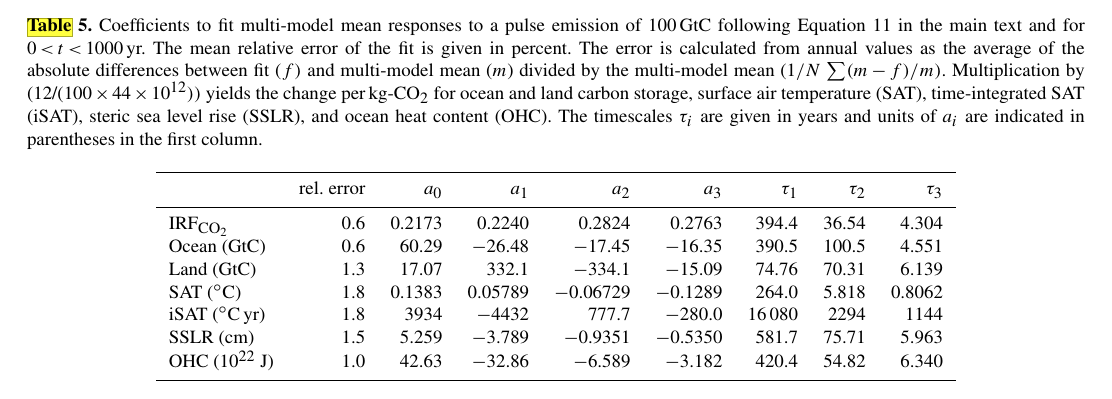
\includegraphics{Joos_CO2_coeffs.png} Ref: Values taken from
\cite{joos_carbon_2013}

    \hypertarget{code-for-calculating-delta-t_co_2}{%
\subsubsection{\texorpdfstring{Code for calculating \(\Delta\)
T\(_{CO_2}\)}{Code for calculating \textbackslash Delta T\_\{CO\_2\}}}\label{code-for-calculating-delta-t_co_2}}

    \begin{tcolorbox}[breakable, size=fbox, boxrule=1pt, pad at break*=1mm,colback=cellbackground, colframe=cellborder]
\prompt{In}{incolor}{10}{\boxspacing}
\begin{Verbatim}[commandchars=\\\{\}]
\PY{n}{alphas\PYZus{}irfco2} \PY{o}{=} \PY{p}{[}\PY{l+m+mf}{0.2173}\PY{p}{,} \PY{l+m+mf}{0.2240}\PY{p}{,} \PY{l+m+mf}{0.2824}\PY{p}{,} \PY{l+m+mf}{0.2763}\PY{p}{]}
\PY{n}{taus\PYZus{}irfco2} \PY{o}{=} \PY{p}{[}\PY{l+m+mf}{394.4}\PY{p}{,} \PY{l+m+mf}{36.54}\PY{p}{,} \PY{l+m+mf}{4.304}\PY{p}{]}


\PY{c+c1}{\PYZsh{} def delta\PYZus{}T(t, r0, tau, tau1=tau1, tau2=tau2, alpha1=c1/tau1, alpha2=c2/tau2):}
\PY{k}{def} \PY{n+nf}{deltaT\PYZus{}co2}\PY{p}{(}\PY{n}{t}\PY{p}{,} \PY{n}{dE}\PY{p}{,} \PY{n}{alphs\PYZus{}co2}\PY{o}{=}\PY{n}{alphas\PYZus{}irfco2}\PY{p}{,} \PY{n}{taus\PYZus{}co2}\PY{o}{=}\PY{n}{taus\PYZus{}irfco2}\PY{p}{,} \PY{n}{alphs\PYZus{}irfc}\PY{o}{=}\PY{p}{[}\PY{n}{alpha1\PYZus{}irf}\PY{p}{,} \PY{n}{alpha2\PYZus{}irf}\PY{p}{]}\PY{p}{,} \PY{n}{taus\PYZus{}ifrc}\PY{o}{=}\PY{p}{[}\PY{n}{tau1\PYZus{}irf}\PY{p}{,} \PY{n}{tau2\PYZus{}irf}\PY{p}{]}\PY{p}{)}\PY{p}{:}
    \PY{l+s+sd}{\PYZdq{}\PYZdq{}\PYZdq{}}
\PY{l+s+sd}{    Calculates delta T for CO2 based on analytic solution}
\PY{l+s+sd}{    :param t: time}
\PY{l+s+sd}{    :param dE: change in emissions}
\PY{l+s+sd}{    :param alphs\PYZus{}co2: alpha values co2 IRF}
\PY{l+s+sd}{    :param taus\PYZus{}co2: tau values co2 IRF}
\PY{l+s+sd}{    :param alphs\PYZus{}irfc: alpha values climate IRF}
\PY{l+s+sd}{    :param taus\PYZus{}ifrc: tau values climate IRF}
\PY{l+s+sd}{    :return:}
\PY{l+s+sd}{    \PYZdq{}\PYZdq{}\PYZdq{}}
    \PY{n}{a0\PYZus{}c} \PY{o}{=} \PY{n}{alphs\PYZus{}co2}\PY{p}{[}\PY{l+m+mi}{0}\PY{p}{]}
    \PY{n}{int1} \PY{o}{=} \PY{n}{I1}\PY{p}{(}\PY{n}{t}\PY{p}{,} \PY{n}{a0}\PY{o}{=}\PY{n}{a0\PYZus{}c}\PY{p}{,} \PY{n}{alphajs\PYZus{}k}\PY{o}{=}\PY{n}{alphs\PYZus{}irfc}\PY{p}{,} \PY{n}{taujs\PYZus{}k}\PY{o}{=}\PY{n}{taus\PYZus{}ifrc}\PY{p}{)}
    \PY{n}{int2} \PY{o}{=} \PY{n}{I2}\PY{p}{(}\PY{n}{t}\PY{p}{,} \PY{n}{alphs\PYZus{}co2}\PY{o}{=}\PY{n}{alphs\PYZus{}co2}\PY{p}{,} \PY{n}{taus\PYZus{}co2}\PY{o}{=}\PY{n}{taus\PYZus{}co2}\PY{p}{,} \PY{n}{alphs\PYZus{}irfc}\PY{o}{=}\PY{n}{alphs\PYZus{}irfc}\PY{p}{,} \PY{n}{taus\PYZus{}irfc}\PY{o}{=}\PY{n}{taus\PYZus{}ifrc}\PY{p}{)}
    \PY{k}{return} \PY{n}{dE} \PY{o}{*} \PY{p}{(}\PY{n}{int2} \PY{o}{+} \PY{n}{int1}\PY{p}{)}


\PY{k}{def} \PY{n+nf}{I2}\PY{p}{(}\PY{n}{t}\PY{p}{,} \PY{n}{alphs\PYZus{}co2} \PY{o}{=} \PY{n}{alphas\PYZus{}irfco2}\PY{p}{,} \PY{n}{taus\PYZus{}co2} \PY{o}{=} \PY{n}{taus\PYZus{}irfco2}\PY{p}{,}
       \PY{n}{alphs\PYZus{}irfc}\PY{o}{=}\PY{p}{[}\PY{n}{alpha1\PYZus{}irf}\PY{p}{,} \PY{n}{alpha2\PYZus{}irf}\PY{p}{]}\PY{p}{,} \PY{n}{taus\PYZus{}irfc}\PY{o}{=}\PY{p}{[}\PY{n}{tau1\PYZus{}irf}\PY{p}{,} \PY{n}{tau2\PYZus{}irf}\PY{p}{]}\PY{p}{)}\PY{p}{:}
    \PY{l+s+sd}{\PYZdq{}\PYZdq{}\PYZdq{}}
\PY{l+s+sd}{    Integral part 2}
\PY{l+s+sd}{    :param t: time}
\PY{l+s+sd}{    :param as\PYZus{}co2: alpha values co2 IRF}
\PY{l+s+sd}{    :param taus\PYZus{}co2: tau values co2 IRF}
\PY{l+s+sd}{    :param alphs\PYZus{}irfc: alpha values climate IRF}
\PY{l+s+sd}{    :param taus\PYZus{}irfc: tau values climate IRF}
\PY{l+s+sd}{    :return: value}
\PY{l+s+sd}{    \PYZdq{}\PYZdq{}\PYZdq{}}
    \PY{n}{ais\PYZus{}c} \PY{o}{=} \PY{n}{alphs\PYZus{}co2}\PY{p}{[}\PY{l+m+mi}{1}\PY{p}{:}\PY{p}{]}
    \PY{n}{tauis\PYZus{}c} \PY{o}{=} \PY{n}{taus\PYZus{}co2}\PY{p}{[}\PY{p}{:}\PY{p}{]}
    \PY{n}{alphajs\PYZus{}k} \PY{o}{=} \PY{n}{alphs\PYZus{}irfc}\PY{p}{[}\PY{p}{:}\PY{p}{]}
    \PY{n}{taujs\PYZus{}k} \PY{o}{=} \PY{n}{taus\PYZus{}irfc}\PY{p}{[}\PY{p}{:}\PY{p}{]}  \PY{c+c1}{\PYZsh{} t,a0 = as\PYZus{}co2[0], alphajs\PYZus{}k = [alpha1\PYZus{}k, alpha2\PYZus{}k], taujs\PYZus{}k = [tau1\PYZus{}k, tau2\PYZus{}k]):}
    \PY{n}{\PYZus{}s1} \PY{o}{=} \PY{l+m+mi}{0}
    \PY{k}{for} \PY{n}{taui}\PY{p}{,} \PY{n}{ai} \PY{o+ow}{in} \PY{n+nb}{zip}\PY{p}{(}\PY{n}{tauis\PYZus{}c}\PY{p}{,} \PY{n}{ais\PYZus{}c}\PY{p}{)}\PY{p}{:}
        \PY{k}{for} \PY{n}{tauj}\PY{p}{,} \PY{n}{alphaj} \PY{o+ow}{in} \PY{n+nb}{zip}\PY{p}{(}\PY{n}{taujs\PYZus{}k}\PY{p}{,} \PY{n}{alphajs\PYZus{}k}\PY{p}{)}\PY{p}{:}
            \PY{n}{\PYZus{}rat} \PY{o}{=} \PY{n}{taui} \PY{o}{/} \PY{p}{(}\PY{n}{tauj} \PY{o}{\PYZhy{}} \PY{n}{taui}\PY{p}{)}
            \PY{n}{\PYZus{}d} \PY{o}{=} \PY{l+m+mi}{1} \PY{o}{\PYZhy{}} \PY{n}{np}\PY{o}{.}\PY{n}{exp}\PY{p}{(}\PY{o}{\PYZhy{}}\PY{n}{t} \PY{o}{/} \PY{n}{tauj}\PY{p}{)} \PY{o}{+} \PY{n}{\PYZus{}rat} \PY{o}{*} \PY{p}{(}\PY{n}{np}\PY{o}{.}\PY{n}{exp}\PY{p}{(}\PY{o}{\PYZhy{}}\PY{n}{t} \PY{o}{/} \PY{n}{taui}\PY{p}{)} \PY{o}{\PYZhy{}} \PY{n}{np}\PY{o}{.}\PY{n}{exp}\PY{p}{(}\PY{o}{\PYZhy{}}\PY{n}{t} \PY{o}{/} \PY{n}{tauj}\PY{p}{)}\PY{p}{)}
            \PY{n}{\PYZus{}s1} \PY{o}{+}\PY{o}{=} \PY{n}{ai} \PY{o}{*} \PY{n}{taui} \PY{o}{*} \PY{n}{alphaj} \PY{o}{*} \PY{n}{tauj} \PY{o}{*} \PY{n}{\PYZus{}d}
    \PY{k}{return} \PY{n}{\PYZus{}s1}


\PY{k}{def} \PY{n+nf}{I1}\PY{p}{(}\PY{n}{t}\PY{p}{,} \PY{n}{a0}\PY{o}{=}\PY{n}{alphas\PYZus{}irfco2}\PY{p}{[}\PY{l+m+mi}{0}\PY{p}{]}\PY{p}{,} \PY{n}{alphajs\PYZus{}k}\PY{o}{=}\PY{p}{[}\PY{n}{alpha1\PYZus{}irf}\PY{p}{,} \PY{n}{alpha2\PYZus{}irf}\PY{p}{]}\PY{p}{,} \PY{n}{taujs\PYZus{}k}\PY{o}{=}\PY{p}{[}\PY{n}{tau1\PYZus{}irf}\PY{p}{,} \PY{n}{tau2\PYZus{}irf}\PY{p}{]}\PY{p}{)}\PY{p}{:}
    \PY{l+s+sd}{\PYZdq{}\PYZdq{}\PYZdq{}}
\PY{l+s+sd}{    Integral part 1}
\PY{l+s+sd}{    :param t: years}
\PY{l+s+sd}{    :param a0: a0 co2 irf}
\PY{l+s+sd}{    :param alphajs\PYZus{}k: alpha values climate IRF}
\PY{l+s+sd}{    :param taujs\PYZus{}k: tau  values climate IRF}
\PY{l+s+sd}{    :return: value of integral}
\PY{l+s+sd}{    \PYZdq{}\PYZdq{}\PYZdq{}}
    \PY{n}{\PYZus{}s1} \PY{o}{=} \PY{l+m+mi}{0}
    \PY{k}{for} \PY{n}{alphaj}\PY{p}{,} \PY{n}{tauj} \PY{o+ow}{in} \PY{n+nb}{zip}\PY{p}{(}\PY{n}{alphajs\PYZus{}k}\PY{p}{,} \PY{n}{taujs\PYZus{}k}\PY{p}{)}\PY{p}{:}
        \PY{n}{\PYZus{}s1} \PY{o}{+}\PY{o}{=} \PY{n}{alphaj} \PY{o}{*} \PY{n}{tauj}
    \PY{n}{\PYZus{}s2} \PY{o}{=} \PY{l+m+mi}{0}
    \PY{k}{for} \PY{n}{alphaj}\PY{p}{,} \PY{n}{tauj} \PY{o+ow}{in} \PY{n+nb}{zip}\PY{p}{(}\PY{n}{alphajs\PYZus{}k}\PY{p}{,} \PY{n}{taujs\PYZus{}k}\PY{p}{)}\PY{p}{:}
        \PY{n}{\PYZus{}s2} \PY{o}{+}\PY{o}{=} \PY{n}{alphaj} \PY{o}{*} \PY{n}{tauj} \PY{o}{*}\PY{o}{*} \PY{l+m+mi}{2} \PY{o}{*} \PY{p}{(}\PY{l+m+mi}{1} \PY{o}{\PYZhy{}} \PY{n}{np}\PY{o}{.}\PY{n}{exp}\PY{p}{(}\PY{o}{\PYZhy{}}\PY{n}{t} \PY{o}{/} \PY{n}{tauj}\PY{p}{)}\PY{p}{)}

    \PY{k}{return} \PY{n}{a0} \PY{o}{*} \PY{p}{(}\PY{n}{t} \PY{o}{*} \PY{n}{\PYZus{}s1} \PY{o}{\PYZhy{}} \PY{n}{\PYZus{}s2}\PY{p}{)}
\end{Verbatim}
\end{tcolorbox}

    \hypertarget{check-correctness-of-integral}{%
\paragraph{Check correctness of
integral}\label{check-correctness-of-integral}}

    \begin{tcolorbox}[breakable, size=fbox, boxrule=1pt, pad at break*=1mm,colback=cellbackground, colframe=cellborder]
\prompt{In}{incolor}{11}{\boxspacing}
\begin{Verbatim}[commandchars=\\\{\}]
\PY{k+kn}{from} \PY{n+nn}{scipy}\PY{n+nn}{.}\PY{n+nn}{integrate} \PY{k+kn}{import} \PY{n}{quad}


\PY{k}{def} \PY{n+nf}{integrand}\PY{p}{(}\PY{n}{t}\PY{p}{,} \PY{n}{tn}\PY{p}{,} \PY{n}{dE}\PY{p}{,} \PY{n}{alphs\PYZus{}co2}\PY{o}{=}\PY{n}{alphas\PYZus{}irfco2}\PY{p}{,} \PY{n}{taus\PYZus{}co2}\PY{o}{=}\PY{n}{taus\PYZus{}irfco2}\PY{p}{,} \PY{n}{a\PYZus{}k}\PY{o}{=}\PY{p}{[}\PY{n}{alpha1\PYZus{}irf}\PY{p}{,} \PY{n}{alpha2\PYZus{}irf}\PY{p}{]}\PY{p}{,} \PY{n}{tau\PYZus{}k}\PY{o}{=}\PY{p}{[}\PY{n}{tau1\PYZus{}irf}\PY{p}{,} \PY{n}{tau2\PYZus{}irf}\PY{p}{]}\PY{p}{)}\PY{p}{:}
    \PY{l+s+sd}{\PYZdq{}\PYZdq{}\PYZdq{}}
\PY{l+s+sd}{    The integrand:}
\PY{l+s+sd}{    RF\PYZus{}\PYZob{}CO\PYZus{}2\PYZcb{}(t\PYZsq{}) * IRF\PYZus{}\PYZob{}Climate\PYZcb{}(t\PYZhy{}t\PYZsq{})}
\PY{l+s+sd}{    :param t: t\PYZsq{}}
\PY{l+s+sd}{    :param tn: t limit}
\PY{l+s+sd}{    :param dE: delta Emissions}
\PY{l+s+sd}{    :param alphs\PYZus{}co2: alpha values co2}
\PY{l+s+sd}{    :param taus\PYZus{}co2: tau values co2}
\PY{l+s+sd}{    :param a\PYZus{}k: alpha values irf climate}
\PY{l+s+sd}{    :param tau\PYZus{}k: tau values irf climate}
\PY{l+s+sd}{    :return: value of integrand}
\PY{l+s+sd}{    \PYZdq{}\PYZdq{}\PYZdq{}}
    \PY{n}{a0\PYZus{}c} \PY{o}{=} \PY{n}{alphas\PYZus{}irfco2}\PY{p}{[}\PY{l+m+mi}{0}\PY{p}{]}
    \PY{n}{ais\PYZus{}c} \PY{o}{=} \PY{n}{alphs\PYZus{}co2}\PY{p}{[}\PY{l+m+mi}{1}\PY{p}{:}\PY{p}{]}
    \PY{n}{tauis\PYZus{}c} \PY{o}{=} \PY{n}{taus\PYZus{}co2}\PY{p}{[}\PY{p}{:}\PY{p}{]}
    \PY{n}{alphajs\PYZus{}k} \PY{o}{=} \PY{n}{a\PYZus{}k}\PY{p}{[}\PY{p}{:}\PY{p}{]}
    \PY{n}{taujs\PYZus{}k} \PY{o}{=} \PY{n}{tau\PYZus{}k}\PY{p}{[}\PY{p}{:}\PY{p}{]}
    \PY{n}{\PYZus{}s} \PY{o}{=} \PY{l+m+mi}{0}
    \PY{k}{for} \PY{n}{taui}\PY{p}{,} \PY{n}{ai} \PY{o+ow}{in} \PY{n+nb}{zip}\PY{p}{(}\PY{n}{tauis\PYZus{}c}\PY{p}{,} \PY{n}{ais\PYZus{}c}\PY{p}{)}\PY{p}{:}
        \PY{n}{\PYZus{}s} \PY{o}{+}\PY{o}{=} \PY{n}{ai} \PY{o}{*} \PY{n}{taui} \PY{o}{*} \PY{p}{(}\PY{l+m+mi}{1} \PY{o}{\PYZhy{}} \PY{n}{np}\PY{o}{.}\PY{n}{exp}\PY{p}{(}\PY{o}{\PYZhy{}}\PY{n}{t} \PY{o}{/} \PY{n}{taui}\PY{p}{)}\PY{p}{)}
    \PY{n}{fact1} \PY{o}{=} \PY{n}{a0\PYZus{}c} \PY{o}{*} \PY{n}{t} \PY{o}{+} \PY{n}{\PYZus{}s}
    \PY{n}{fact2} \PY{o}{=} \PY{n}{alphajs\PYZus{}k}\PY{p}{[}\PY{l+m+mi}{0}\PY{p}{]} \PY{o}{*} \PY{n}{np}\PY{o}{.}\PY{n}{exp}\PY{p}{(}\PY{o}{\PYZhy{}}\PY{p}{(}\PY{n}{tn} \PY{o}{\PYZhy{}} \PY{n}{t}\PY{p}{)} \PY{o}{/} \PY{n}{taujs\PYZus{}k}\PY{p}{[}\PY{l+m+mi}{0}\PY{p}{]}\PY{p}{)} \PY{o}{+} \PY{n}{alphajs\PYZus{}k}\PY{p}{[}\PY{l+m+mi}{1}\PY{p}{]} \PY{o}{*} \PY{n}{np}\PY{o}{.}\PY{n}{exp}\PY{p}{(}\PY{o}{\PYZhy{}}\PY{p}{(}\PY{n}{tn} \PY{o}{\PYZhy{}} \PY{n}{t}\PY{p}{)} \PY{o}{/} \PY{n}{taujs\PYZus{}k}\PY{p}{[}\PY{l+m+mi}{1}\PY{p}{]}\PY{p}{)}
    \PY{k}{return} \PY{n}{dE} \PY{o}{*} \PY{p}{(}\PY{n}{fact1} \PY{o}{*} \PY{n}{fact2}\PY{p}{)}


\PY{n}{integ} \PY{o}{=} \PY{p}{[}\PY{p}{]}

\PY{k}{for} \PY{n}{t} \PY{o+ow}{in} \PY{n}{t\PYZus{}yrs}\PY{p}{:}
    \PY{c+c1}{\PYZsh{} Numerically integrate:}
    \PY{n}{integ}\PY{o}{.}\PY{n}{append}\PY{p}{(}\PY{n}{quad}\PY{p}{(}\PY{n}{integrand}\PY{p}{,} \PY{l+m+mi}{0}\PY{p}{,} \PY{n}{t}\PY{p}{,} \PY{n}{args}\PY{o}{=}\PY{p}{(}\PY{n}{t}\PY{p}{,} \PY{n}{delta\PYZus{}E}\PY{p}{(}\PY{p}{)}\PY{p}{)}\PY{p}{)}\PY{p}{[}\PY{l+m+mi}{0}\PY{p}{]}\PY{p}{)}
\PY{n}{plt}\PY{o}{.}\PY{n}{plot}\PY{p}{(}\PY{n}{t\PYZus{}yrs}\PY{p}{,} \PY{n}{integ}\PY{p}{)}
\PY{n}{y} \PY{o}{=} \PY{n}{deltaT\PYZus{}co2}\PY{p}{(}\PY{n}{t\PYZus{}yrs}\PY{p}{,} \PY{n}{delta\PYZus{}E}\PY{p}{(}\PY{p}{)}\PY{p}{)}
\PY{n}{plt}\PY{o}{.}\PY{n}{plot}\PY{p}{(}\PY{n}{t\PYZus{}yrs}\PY{p}{,} \PY{n}{y}\PY{p}{,} \PY{n}{linestyle}\PY{o}{=}\PY{l+s+s1}{\PYZsq{}}\PY{l+s+s1}{dashed}\PY{l+s+s1}{\PYZsq{}}\PY{p}{)}
\PY{n}{plt}\PY{o}{.}\PY{n}{show}\PY{p}{(}\PY{p}{)}
\end{Verbatim}
\end{tcolorbox}

    \begin{figure}
        \begin{center}\adjustimage{max size={0.9\linewidth}{0.4\paperheight}}{delta_T_CO2_plots_final_files/delta_T_CO2_plots_final_52_0.png}\end{center}
        \caption{}
        \label{}
    \end{figure}
    
    \hypertarget{final-combined-plots}{%
\section{Final combined plots:}\label{final-combined-plots}}

    \begin{tcolorbox}[breakable, size=fbox, boxrule=1pt, pad at break*=1mm,colback=cellbackground, colframe=cellborder]
\prompt{In}{incolor}{12}{\boxspacing}
\begin{Verbatim}[commandchars=\\\{\}]
\PY{k}{def} \PY{n+nf}{set\PYZus{}fontsize}\PY{p}{(}\PY{n}{ax}\PY{p}{,} \PY{n}{SM}\PY{o}{=}\PY{l+m+mi}{8}\PY{p}{,} \PY{n}{MED}\PY{o}{=}\PY{l+m+mi}{10}\PY{p}{,} \PY{n}{BIG}\PY{o}{=}\PY{l+m+mi}{12}\PY{p}{)}\PY{p}{:}
    \PY{c+c1}{\PYZsh{} ax.title.set\PYZus{}fontsize(SM)}
    \PY{k}{for} \PY{n}{item} \PY{o+ow}{in} \PY{p}{[}\PY{n}{ax}\PY{o}{.}\PY{n}{title}\PY{p}{,} \PY{n}{ax}\PY{o}{.}\PY{n}{xaxis}\PY{o}{.}\PY{n}{label}\PY{p}{,} \PY{n}{ax}\PY{o}{.}\PY{n}{yaxis}\PY{o}{.}\PY{n}{label}\PY{p}{]}\PY{p}{:}
        \PY{n}{item}\PY{o}{.}\PY{n}{set\PYZus{}fontsize}\PY{p}{(}\PY{n}{SM}\PY{p}{)}
    \PY{n}{ax}\PY{o}{.}\PY{n}{title}\PY{o}{.}\PY{n}{set\PYZus{}fontsize}\PY{p}{(}\PY{n}{SM}\PY{p}{)}

    \PY{k}{for} \PY{n}{item} \PY{o+ow}{in} \PY{p}{(}\PY{n}{ax}\PY{o}{.}\PY{n}{get\PYZus{}xticklabels}\PY{p}{(}\PY{p}{)} \PY{o}{+} \PY{n}{ax}\PY{o}{.}\PY{n}{get\PYZus{}yticklabels}\PY{p}{(}\PY{p}{)}\PY{p}{)}\PY{p}{:}
        \PY{n}{item}\PY{o}{.}\PY{n}{set\PYZus{}fontsize}\PY{p}{(}\PY{n}{SM}\PY{p}{)}
\end{Verbatim}
\end{tcolorbox}

    \begin{tcolorbox}[breakable, size=fbox, boxrule=1pt, pad at break*=1mm,colback=cellbackground, colframe=cellborder]
\prompt{In}{incolor}{13}{\boxspacing}
\begin{Verbatim}[commandchars=\\\{\}]
\PY{k+kn}{import} \PY{n+nn}{matplotlib}\PY{n+nn}{.}\PY{n+nn}{pyplot} \PY{k}{as} \PY{n+nn}{plt}
\PY{k+kn}{from} \PY{n+nn}{mpl\PYZus{}toolkits}\PY{n+nn}{.}\PY{n+nn}{axes\PYZus{}grid1}\PY{n+nn}{.}\PY{n+nn}{inset\PYZus{}locator} \PY{k+kn}{import} \PY{n}{TransformedBbox}\PY{p}{,} \PY{n}{BboxPatch}\PY{p}{,} \PY{n}{BboxConnector} 
\PY{k+kn}{import} \PY{n+nn}{numpy} \PY{k}{as} \PY{n+nn}{np}
\end{Verbatim}
\end{tcolorbox}

    \begin{tcolorbox}[breakable, size=fbox, boxrule=1pt, pad at break*=1mm,colback=cellbackground, colframe=cellborder]
\prompt{In}{incolor}{14}{\boxspacing}
\begin{Verbatim}[commandchars=\\\{\}]
\PY{k}{def} \PY{n+nf}{mark\PYZus{}inset}\PY{p}{(}\PY{n}{parent\PYZus{}axes}\PY{p}{,} \PY{n}{inset\PYZus{}axes}\PY{p}{,} \PY{n}{loc1a}\PY{o}{=}\PY{l+m+mi}{1}\PY{p}{,} \PY{n}{loc1b}\PY{o}{=}\PY{l+m+mi}{1}\PY{p}{,} \PY{n}{loc2a}\PY{o}{=}\PY{l+m+mi}{2}\PY{p}{,} \PY{n}{loc2b}\PY{o}{=}\PY{l+m+mi}{2}\PY{p}{,} \PY{o}{*}\PY{o}{*}\PY{n}{kwargs}\PY{p}{)}\PY{p}{:}
    \PY{n}{rect} \PY{o}{=} \PY{n}{TransformedBbox}\PY{p}{(}\PY{n}{inset\PYZus{}axes}\PY{o}{.}\PY{n}{viewLim}\PY{p}{,} \PY{n}{parent\PYZus{}axes}\PY{o}{.}\PY{n}{transData}\PY{p}{)}

    \PY{n}{pp} \PY{o}{=} \PY{n}{BboxPatch}\PY{p}{(}\PY{n}{rect}\PY{p}{,} \PY{n}{fill}\PY{o}{=}\PY{k+kc}{False}\PY{p}{,} \PY{o}{*}\PY{o}{*}\PY{n}{kwargs}\PY{p}{)}
    \PY{n}{parent\PYZus{}axes}\PY{o}{.}\PY{n}{add\PYZus{}patch}\PY{p}{(}\PY{n}{pp}\PY{p}{)}

    \PY{n}{p1} \PY{o}{=} \PY{n}{BboxConnector}\PY{p}{(}\PY{n}{inset\PYZus{}axes}\PY{o}{.}\PY{n}{bbox}\PY{p}{,} \PY{n}{rect}\PY{p}{,} \PY{n}{loc1}\PY{o}{=}\PY{n}{loc1a}\PY{p}{,} \PY{n}{loc2}\PY{o}{=}\PY{n}{loc1b}\PY{p}{,} \PY{o}{*}\PY{o}{*}\PY{n}{kwargs}\PY{p}{,}
                       
                       
                      \PY{p}{)}
    \PY{n}{inset\PYZus{}axes}\PY{o}{.}\PY{n}{add\PYZus{}patch}\PY{p}{(}\PY{n}{p1}\PY{p}{)}
    \PY{n}{p1}\PY{o}{.}\PY{n}{set\PYZus{}clip\PYZus{}on}\PY{p}{(}\PY{k+kc}{False}\PY{p}{)}
    \PY{n}{p2} \PY{o}{=} \PY{n}{BboxConnector}\PY{p}{(}\PY{n}{inset\PYZus{}axes}\PY{o}{.}\PY{n}{bbox}\PY{p}{,} \PY{n}{rect}\PY{p}{,} \PY{n}{loc1}\PY{o}{=}\PY{n}{loc2a}\PY{p}{,} \PY{n}{loc2}\PY{o}{=}\PY{n}{loc2b}\PY{p}{,} \PY{o}{*}\PY{o}{*}\PY{n}{kwargs}\PY{p}{)}
    \PY{n}{inset\PYZus{}axes}\PY{o}{.}\PY{n}{add\PYZus{}patch}\PY{p}{(}\PY{n}{p2}\PY{p}{)}
    \PY{n}{p2}\PY{o}{.}\PY{n}{set\PYZus{}clip\PYZus{}on}\PY{p}{(}\PY{k+kc}{False}\PY{p}{)}

    \PY{k}{return} \PY{n}{pp}\PY{p}{,} \PY{n}{p1}\PY{p}{,} \PY{n}{p2}

\PY{c+c1}{\PYZsh{}mark\PYZus{}inset(ax, axins, loc1a=1, loc1b=4, loc2a=2, loc2b=3, fc=\PYZdq{}none\PYZdq{}, ec=\PYZdq{}crimson\PYZdq{}) }
\end{Verbatim}
\end{tcolorbox}

    \begin{tcolorbox}[breakable, size=fbox, boxrule=1pt, pad at break*=1mm,colback=cellbackground, colframe=cellborder]
\prompt{In}{incolor}{15}{\boxspacing}
\begin{Verbatim}[commandchars=\\\{\}]
\PY{k+kn}{import} \PY{n+nn}{matplotlib}\PY{n+nn}{.}\PY{n+nn}{pyplot} \PY{k}{as} \PY{n+nn}{plt}

\PY{k+kn}{from} \PY{n+nn}{mpl\PYZus{}toolkits}\PY{n+nn}{.}\PY{n+nn}{axes\PYZus{}grid1}\PY{n+nn}{.}\PY{n+nn}{inset\PYZus{}locator} \PY{k+kn}{import} \PY{n}{zoomed\PYZus{}inset\PYZus{}axes}
\PY{c+c1}{\PYZsh{}from mpl\PYZus{}toolkits.axes\PYZus{}grid1.inset\PYZus{}locator import mark\PYZus{}inset}

\PY{k+kn}{import} \PY{n+nn}{numpy} \PY{k}{as} \PY{n+nn}{np}


\PY{c+c1}{\PYZsh{}fig, ax\PYZus{}short = plt.subplots(figsize=[5,2])}
\PY{n}{fig}\PY{p}{,} \PY{n}{ax\PYZus{}short} \PY{o}{=} \PY{n}{plt}\PY{o}{.}\PY{n}{subplots}\PY{p}{(} \PY{n}{figsize}\PY{o}{=}\PY{p}{[}\PY{l+m+mi}{6}\PY{p}{,} \PY{l+m+mi}{6}\PY{p}{]}\PY{p}{,} \PY{n}{dpi}\PY{o}{=}\PY{l+m+mi}{150}\PY{p}{)}


  
\PY{c+c1}{\PYZsh{}ax.plot(x, y)}

\PY{n}{ax\PYZus{}long} \PY{o}{=} \PY{n}{ax\PYZus{}short}\PY{o}{.}\PY{n}{inset\PYZus{}axes}\PY{p}{(}\PY{p}{[}\PY{o}{.}\PY{l+m+mi}{0}\PY{p}{,} \PY{o}{\PYZhy{}}\PY{o}{.}\PY{l+m+mi}{6}\PY{p}{,} \PY{o}{.}\PY{l+m+mi}{6}\PY{p}{,} \PY{o}{.}\PY{l+m+mi}{4}\PY{p}{]}\PY{p}{,} \PY{n}{facecolor}\PY{o}{=}\PY{l+s+s1}{\PYZsq{}}\PY{l+s+s1}{w}\PY{l+s+s1}{\PYZsq{}}\PY{p}{,} \PY{n}{frameon}\PY{o}{=}\PY{k+kc}{True}\PY{p}{)}\PY{c+c1}{\PYZsh{}[.8,.6,.4,.4])\PYZsh{}zoomed\PYZus{}inset\PYZus{}axes(ax\PYZus{}long, 20, loc=\PYZsq{}center right\PYZsq{}, bbox\PYZus{}to\PYZus{}anchor=(1,1)) \PYZsh{} zoom = 6}

\PY{c+c1}{\PYZsh{}ax\PYZus{}long = plt.axes([.65, .6, .3, .25], facecolor=\PYZsq{}w\PYZsq{}, frameon=True)  \PYZsh{} , fontsize=10)}

\PY{k}{for} \PY{n}{ax} \PY{o+ow}{in} \PY{p}{[}\PY{n}{ax\PYZus{}short}\PY{p}{,} \PY{n}{ax\PYZus{}long}\PY{p}{]}\PY{p}{:}
    \PY{c+c1}{\PYZsh{} plot standard agents}
    \PY{n}{df}\PY{o}{.}\PY{n}{plot}\PY{o}{.}\PY{n}{line}\PY{p}{(}\PY{n}{ax}\PY{o}{=}\PY{n}{ax}\PY{p}{,} \PY{n}{legend}\PY{o}{=}\PY{k+kc}{False}\PY{p}{,} \PY{n}{cmap}\PY{o}{=}\PY{l+s+s1}{\PYZsq{}}\PY{l+s+s1}{viridis}\PY{l+s+s1}{\PYZsq{}}\PY{p}{)}\PY{c+c1}{\PYZsh{}, linewidth=linewid[ax])}
    \PY{n}{y} \PY{o}{=} \PY{n}{deltaT\PYZus{}co2}\PY{p}{(}\PY{n}{t\PYZus{}yrs}\PY{p}{,} \PY{n}{delta\PYZus{}E}\PY{p}{(}\PY{p}{)}\PY{p}{)}  \PY{c+c1}{\PYZsh{} a\PYZus{}vals=\PYZus{}a, t=1e100))}
    \PY{n}{ax}\PY{o}{.}\PY{n}{plot}\PY{p}{(}\PY{n}{t\PYZus{}yrs}\PY{p}{,} \PY{n}{y}\PY{p}{,} \PY{n}{label}\PY{o}{=}\PY{l+s+s1}{\PYZsq{}}\PY{l+s+s1}{CO\PYZdl{}\PYZus{}2\PYZdl{}}\PY{l+s+s1}{\PYZsq{}}\PY{p}{,} \PY{n}{c}\PY{o}{=}\PY{l+s+s1}{\PYZsq{}}\PY{l+s+s1}{k}\PY{l+s+s1}{\PYZsq{}}\PY{p}{,} \PY{n}{linestyle}\PY{o}{=}\PY{l+s+s1}{\PYZsq{}}\PY{l+s+s1}{dashed}\PY{l+s+s1}{\PYZsq{}}\PY{p}{)}
    \PY{c+c1}{\PYZsh{}, linewidth=linewid[ax])}
\PY{c+c1}{\PYZsh{}axins.plot(x, y)}
\PY{n}{ax\PYZus{}short}\PY{o}{.}\PY{n}{set\PYZus{}xlim}\PY{p}{(}\PY{p}{[}\PY{l+m+mi}{0}\PY{p}{,} \PY{l+m+mi}{100}\PY{p}{]}\PY{p}{)} \PY{c+c1}{\PYZsh{} Limit the region for zoom}
\PY{n}{ax\PYZus{}short}\PY{o}{.}\PY{n}{set\PYZus{}ylim}\PY{p}{(}\PY{p}{[}\PY{o}{\PYZhy{}}\PY{o}{.}\PY{l+m+mi}{55}\PY{p}{,} \PY{o}{.}\PY{l+m+mi}{2}\PY{p}{]}\PY{p}{)}
\PY{n}{ax\PYZus{}long}\PY{o}{.}\PY{n}{set\PYZus{}xlim}\PY{p}{(}\PY{p}{[}\PY{o}{\PYZhy{}}\PY{l+m+mi}{1}\PY{p}{,}\PY{l+m+mi}{400}\PY{p}{]}\PY{p}{)} \PY{c+c1}{\PYZsh{} Limit the region for zoom}
\PY{n}{ax\PYZus{}long}\PY{o}{.}\PY{n}{set\PYZus{}ylim}\PY{p}{(}\PY{p}{[}\PY{o}{\PYZhy{}}\PY{l+m+mi}{2}\PY{p}{,} \PY{o}{.}\PY{l+m+mi}{22}\PY{p}{]}\PY{p}{)}

\PY{c+c1}{\PYZsh{}\PYZsh{} draw a bbox of the region of the inset axes in the parent axes and}
\PY{c+c1}{\PYZsh{}\PYZsh{} connecting lines between the bbox and the inset axes area}
\PY{n}{mark\PYZus{}inset}\PY{p}{(}\PY{n}{ax}\PY{p}{,} \PY{n}{ax\PYZus{}short}\PY{p}{,} \PY{n}{loc1b}\PY{o}{=}\PY{l+m+mi}{1}\PY{p}{,} \PY{n}{loc1a}\PY{o}{=}\PY{l+m+mi}{4}\PY{p}{,} \PY{n}{loc2b}\PY{o}{=}\PY{l+m+mi}{2}\PY{p}{,} \PY{n}{loc2a}\PY{o}{=}\PY{l+m+mi}{3}\PY{p}{,}  
           \PY{n}{fc}\PY{o}{=}\PY{l+s+s2}{\PYZdq{}}\PY{l+s+s2}{none}\PY{l+s+s2}{\PYZdq{}}\PY{p}{,}
           \PY{c+c1}{\PYZsh{}linewidth=2, }
           \PY{n}{ec}\PY{o}{=}\PY{l+s+s2}{\PYZdq{}}\PY{l+s+s2}{0.5}\PY{l+s+s2}{\PYZdq{}}\PY{p}{,}
           \PY{n}{zorder}\PY{o}{=}\PY{o}{\PYZhy{}}\PY{l+m+mi}{1}\PY{p}{)}\PY{c+c1}{\PYZsh{}, edgecolor=\PYZsq{}r\PYZsq{})}

\PY{n}{ax\PYZus{}short}\PY{o}{.}\PY{n}{legend}\PY{p}{(}\PY{n}{title}\PY{o}{=}\PY{l+s+s1}{\PYZsq{}}\PY{l+s+s1}{Lifetime}\PY{l+s+s1}{\PYZsq{}}\PY{p}{,}\PY{n}{frameon}\PY{o}{=}\PY{k+kc}{False}\PY{p}{,} \PY{n}{ncol} \PY{o}{=}\PY{l+m+mi}{2}\PY{p}{)}\PY{c+c1}{\PYZsh{}, bbox\PYZus{}to\PYZus{}anchor=(.6,.8))}

\PY{c+c1}{\PYZsh{}plt.draw()}
\PY{c+c1}{\PYZsh{}ax\PYZus{}long.get\PYZus{}legend().remove()  \PYZsh{} legend(visible=False)}
\PY{c+c1}{\PYZsh{}ax\PYZus{}short.set\PYZus{}ylabel(\PYZsq{}Reduced warming (\PYZdl{}\PYZca{}\PYZbs{}circ\PYZdl{}C)\PYZsq{})}
\PY{n}{ax\PYZus{}long}\PY{o}{.}\PY{n}{set\PYZus{}ylabel}\PY{p}{(}\PY{l+s+s1}{\PYZsq{}}\PY{l+s+s1}{(\PYZdl{}\PYZca{}}\PY{l+s+s1}{\PYZbs{}}\PY{l+s+s1}{circ\PYZdl{}C)}\PY{l+s+s1}{\PYZsq{}}\PY{p}{)}
\PY{n}{ax\PYZus{}short}\PY{o}{.}\PY{n}{set\PYZus{}ylabel}\PY{p}{(}\PY{l+s+s1}{\PYZsq{}}\PY{l+s+s1}{(\PYZdl{}\PYZca{}}\PY{l+s+s1}{\PYZbs{}}\PY{l+s+s1}{circ\PYZdl{}C)}\PY{l+s+s1}{\PYZsq{}}\PY{p}{)}
\PY{n}{ax\PYZus{}short}\PY{o}{.}\PY{n}{set\PYZus{}title}\PY{p}{(}\PY{l+s+s1}{\PYZsq{}}\PY{l+s+s1}{Reduced warming after abrupt decrease in SLCFs and CO\PYZdl{}\PYZus{}2\PYZdl{} emissions}\PY{l+s+s1}{\PYZsq{}}\PY{p}{)}
\PY{n}{ax\PYZus{}short}\PY{o}{.}\PY{n}{set\PYZus{}title}\PY{p}{(}\PY{l+s+s1}{\PYZsq{}}\PY{l+s+s1}{Cooling after abrupt reduction in SLCFs and CO\PYZdl{}\PYZus{}2\PYZdl{} emissions}\PY{l+s+s1}{\PYZsq{}}\PY{p}{)}
\PY{c+c1}{\PYZsh{}fig.suptitlele(\PYZsq{}Reduced warming after abrupt decrease in SLCFs and CO\PYZdl{}\PYZus{}2\PYZdl{} emissions\PYZsq{})}
\PY{c+c1}{\PYZsh{}fig.suptitle(\PYZsq{}Reduced warming from mitigation of SLCFs and CO\PYZdl{}\PYZus{}2\PYZdl{}\PYZsq{})}
\PY{n}{ax\PYZus{}long}\PY{o}{.}\PY{n}{set\PYZus{}xlabel}\PY{p}{(}\PY{l+s+s1}{\PYZsq{}}\PY{l+s+s1}{Years since start of emission reduction}\PY{l+s+s1}{\PYZsq{}}\PY{p}{)}
\PY{n}{ax\PYZus{}short}\PY{o}{.}\PY{n}{set\PYZus{}xlabel}\PY{p}{(}\PY{l+s+s1}{\PYZsq{}}\PY{l+s+s1}{\PYZsq{}}\PY{p}{)}\PY{c+c1}{\PYZsh{}Years since start of emission decrease\PYZsq{})}
\PY{c+c1}{\PYZsh{}ax\PYZus{}short.spines[\PYZsq{}right\PYZsq{}].set\PYZus{}visible(False)}
\PY{c+c1}{\PYZsh{}ax\PYZus{}short.spines[\PYZsq{}top\PYZsq{}].set\PYZus{}visible(False)}
\PY{c+c1}{\PYZsh{}ax\PYZus{}long.spines[\PYZsq{}right\PYZsq{}].set\PYZus{}visible(False)}
\PY{c+c1}{\PYZsh{}ax\PYZus{}long.spines[\PYZsq{}top\PYZsq{}].set\PYZus{}visible(False)}
\PY{c+c1}{\PYZsh{}mark\PYZus{}inset(ax, ax\PYZus{}short, loc1=2, loc2=4, fc=\PYZdq{}none\PYZdq{}, ec=\PYZdq{}0.5\PYZdq{})}
\PY{n}{ax\PYZus{}long}\PY{o}{.}\PY{n}{patch}\PY{o}{.}\PY{n}{set\PYZus{}alpha}\PY{p}{(}\PY{l+m+mf}{0.}\PY{p}{)}
\PY{c+c1}{\PYZsh{}ax\PYZus{}long.text(10,\PYZhy{}1.5,\PYZsq{}Long term future\PYZsq{}, alpha=.7)}

\PY{n}{fig}\PY{o}{.}\PY{n}{tight\PYZus{}layout}\PY{p}{(}\PY{p}{)}

\PY{n}{fname} \PY{o}{=} \PY{l+s+s1}{\PYZsq{}}\PY{l+s+s1}{plots/embedded\PYZus{}long\PYZus{}time.}\PY{l+s+s1}{\PYZsq{}}

\PY{c+c1}{\PYZsh{}fig.savefig(fname, dpi=300)}
\PY{c+c1}{\PYZsh{}fig.subplots\PYZus{}adjust(bottom=.1)}

\PY{n}{fig}\PY{o}{.}\PY{n}{savefig}\PY{p}{(}\PY{n}{fname}\PY{o}{+}\PY{l+s+s1}{\PYZsq{}}\PY{l+s+s1}{pdf}\PY{l+s+s1}{\PYZsq{}}\PY{p}{,} \PY{n}{dpi}\PY{o}{=}\PY{l+m+mi}{300}\PY{p}{,}  \PY{n}{bbox\PYZus{}inches} \PY{o}{=} \PY{l+s+s1}{\PYZsq{}}\PY{l+s+s1}{tight}\PY{l+s+s1}{\PYZsq{}}\PY{p}{,} \PY{n}{bbox\PYZus{}extra\PYZus{}artists}\PY{o}{=}\PY{p}{(}\PY{n}{ax\PYZus{}long}\PY{p}{,}\PY{p}{)}\PY{p}{)}
\PY{n}{fig}\PY{o}{.}\PY{n}{savefig}\PY{p}{(}\PY{n}{fname}\PY{o}{+}\PY{l+s+s1}{\PYZsq{}}\PY{l+s+s1}{png}\PY{l+s+s1}{\PYZsq{}}\PY{p}{,} \PY{n}{dpi}\PY{o}{=}\PY{l+m+mi}{300}\PY{p}{,}  \PY{n}{bbox\PYZus{}inches} \PY{o}{=} \PY{l+s+s1}{\PYZsq{}}\PY{l+s+s1}{tight}\PY{l+s+s1}{\PYZsq{}}\PY{p}{,} \PY{n}{bbox\PYZus{}extra\PYZus{}artists}\PY{o}{=}\PY{p}{(}\PY{n}{ax\PYZus{}long}\PY{p}{,}\PY{p}{)}\PY{p}{)}
\PY{n}{plt}\PY{o}{.}\PY{n}{show}\PY{p}{(}\PY{p}{)}
\end{Verbatim}
\end{tcolorbox}

    \begin{figure}
        \begin{center}\adjustimage{max size={0.9\linewidth}{0.4\paperheight}}{delta_T_CO2_plots_final_files/delta_T_CO2_plots_final_57_0.png}\end{center}
        \caption{}
        \label{}
    \end{figure}
    

    % Add a bibliography block to the postdoc
    
    \bibliographystyle{plain}\bibliography{IPCC_terje}

    
\end{document}
